% !TEX TS-program = pdflatexmk
% !TEX root = EUDAQUserManual.tex
\documentclass[12pt, oneside, notitlepage, a4paper]{scrartcl}
\usepackage{epsfig, scrpage2, graphicx, listings, microtype, setspace, upquote}
\usepackage[british]{babel}
\usepackage{hyperref} % must be the last package (apart from glossaries)
\usepackage[toc, nonumberlist]{glossaries} % must go after hyperref, so entries are clickable

\setcounter{secnumdepth}{3}
\setcounter{tocdepth}{2}

\setlength{\parindent}{0em}
\setlength{\parskip}{0ex plus0.5ex minus0ex}
\pagestyle{scrheadings}

\def\subsectionautorefname{section}
\def\subsubsectionautorefname{section}
%\let\stdsection\section
%\renewcommand\section{\newpage\stdsection}

% Some useful commands
\newcommand*\micron{\ensuremath{\mu\mathrm{m}}}
\newcommand*\micro{\ensuremath{\mu}}
\newcommand*\square{\ensuremath{^2}}
\newcommand*\degree{\ensuremath{^\circ}}
\newcommand*\lt{\ensuremath{<}}
\newcommand*\gt{\ensuremath{>}}
\newcommand*\x{\ensuremath{\times}}
\newcommand*\param[1]{\ensuremath{\langle}#1\ensuremath{\rangle}}

\newcommand*\ttitem[1]{\item[\texttt{#1}\,:]}
\newcommand*\ccitem[1]{\item[]\lstinline[style=shaded,language=C++]{#1}}
%\lstMakeShortInline[style=plain,language=C++]@
\newcommand*\inline[2][C++]{\lstinline[style=plain,language=#1]{#2}}

\newcommand*\myinputlisting[3][C++]{
  %% Latest version available at:\\
  %% \textls[#2]{\url{https://github.com/eudaq/eudaq/blob/master/#3}}

\lstinputlisting[style=full, language=#1]{../../#3}
%% \rule[\baselineskip]{\textwidth}{1pt}
}

\lstnewenvironment{listing}[1][C++]{\lstset{style=shaded,language=#1}}{}

\newenvironment{myitemize}
{\begin{itemize}%
  \setlength{\itemsep}{0.1\baselineskip}%
  \setlength{\parskip}{0pt}%
  \setlength{\parsep}{0pt}}
{\end{itemize}}
\newenvironment{mydescription}
{\begin{description}%
  \setlength{\itemsep}{0.1\baselineskip}%
  \setlength{\parskip}{0pt}%
  \setlength{\parsep}{0pt}}
{\end{description}}

\renewcommand*\headfont{\normalfont}

\renewcommand*\glsgroupskip{}
\renewcommand*{\glspostdescription}{.\vspace{-0.5\baselineskip}}
\makeglossaries

%\glsdisablehyper
%\defglsdisplay{\cooltooltip[1,1,0.9][1,1,1]{Glossary}{a #2}{}{b #2}{#1}}
%\renewcommand{\glsdisplay}[4]{%
%   \cooltooltip[1,1,1][1,1,0.9]{Definition}{#2}{}{#2}{#1#4}%
%} 

\lstset{
    %basicstyle=\ttfamily
    keywordstyle=\color[rgb]{0,0,0.8},
    %identifierstyle=\color[rgb]{0,0,0},
    commentstyle=\color[rgb]{0,0.4,0},
    stringstyle=\color[rgb]{0.4,0,0.8},
    showstringspaces=false,
    basewidth=1.2ex,
    numberstyle=\footnotesize\color[rgb]{0.6,0.6,0.6},
    stepnumber=1,
    numbersep=10pt,
    tabsize=2,
    breaklines=true,
    prebreak = \raisebox{0ex}[0ex][0ex]{\color[rgb]{0.6,0.6,0.6}\ensuremath{\hookleftarrow}},
    breakatwhitespace=true,
    %aboveskip={1.5\baselineskip},
    columns=fixed,
    upquote=true,
    extendedchars=false,
    framerule=0pt,
    belowskip={0.5\baselineskip},
}
\lstdefinestyle{plain}{
    basicstyle=\normalsize\ttfamily,
    numbers=none,
    frame=none,
    %belowskip={0.5\baselineskip},
    backgroundcolor={},
}
\lstdefinestyle{shaded}{
    basicstyle=\small\ttfamily,
    numbers=none,
    frame=single,
    backgroundcolor=\color[rgb]{1,0.98,0.95},
}
\lstdefinestyle{full}{
    basicstyle=\small\ttfamily,
    numbers=left,
    frame=single,
    %belowskip={\baselineskip},
    backgroundcolor=\color[rgb]{1,1,0.95},
}

\lstdefinestyle{cpp}{
    language=C++, 
    morekeywords={override, final},
    basicstyle=\small\ttfamily,
    numbers=left,
    frame=single,
    %belowskip={\baselineskip},
    backgroundcolor=\color[rgb]{1,1,0.95},
    %% texcl=true,
    rangeprefix=//----------DOC-MARK-----,
    rangesuffix=-----DOC-MARK----------,
    includerangemarker=false,
    columns=flexible,
    %% escapeinside={//TODO}{.},
}


\lstdefinelanguage{conf}{
    otherkeywords={=},
    alsoletter={[},
    alsoletter={]},
    moredelim=[s][keywordstyle]{[}{]},
    comment=[l]{\#},
    %morecomment=[l]{\;},
    %string=[s]',
    %morestring=[s]",
}
\lstdefinelanguage{mybash}[]{bash}{
    deletekeywords={test,read},
    morekeywords={svn,make,chown,chmod},
    %keywordsprefix={./},
    moredelim=[is][keywordstyle]{$[}{]$},
}


% Insert EUDET document number here:
\newcommand*\EUDETnum{EUDAQ User Manual}

% PDF info and link colours
\hypersetup{
  pdftitle={EUDAQ2 User Manual},
  pdfauthor={EUDAQ Development Team},
  pdfsubject={EUDAQ},
  pdfkeywords={EUDAQ, AIDA, EUDET, Software, User Manual},
  colorlinks=true,
  linkcolor=black, % \ref \autoref \pageref
  citecolor=blue, % \cite
  urlcolor=blue, % \url \href (external)
  filecolor=blue, % \href (local file)
}

% Load glossary
\loadglsentries{src/glossary.tex}

% Headers and Footers
\titlehead{\EUDETnum}
\lehead{\EUDETnum}
\lohead{\EUDETnum}
\automark{section}
\rehead{\headmark}
\rohead{\headmark}
\chead{}
\cfoot{\pagemark}

% Title info
\subject{
\begin{center}
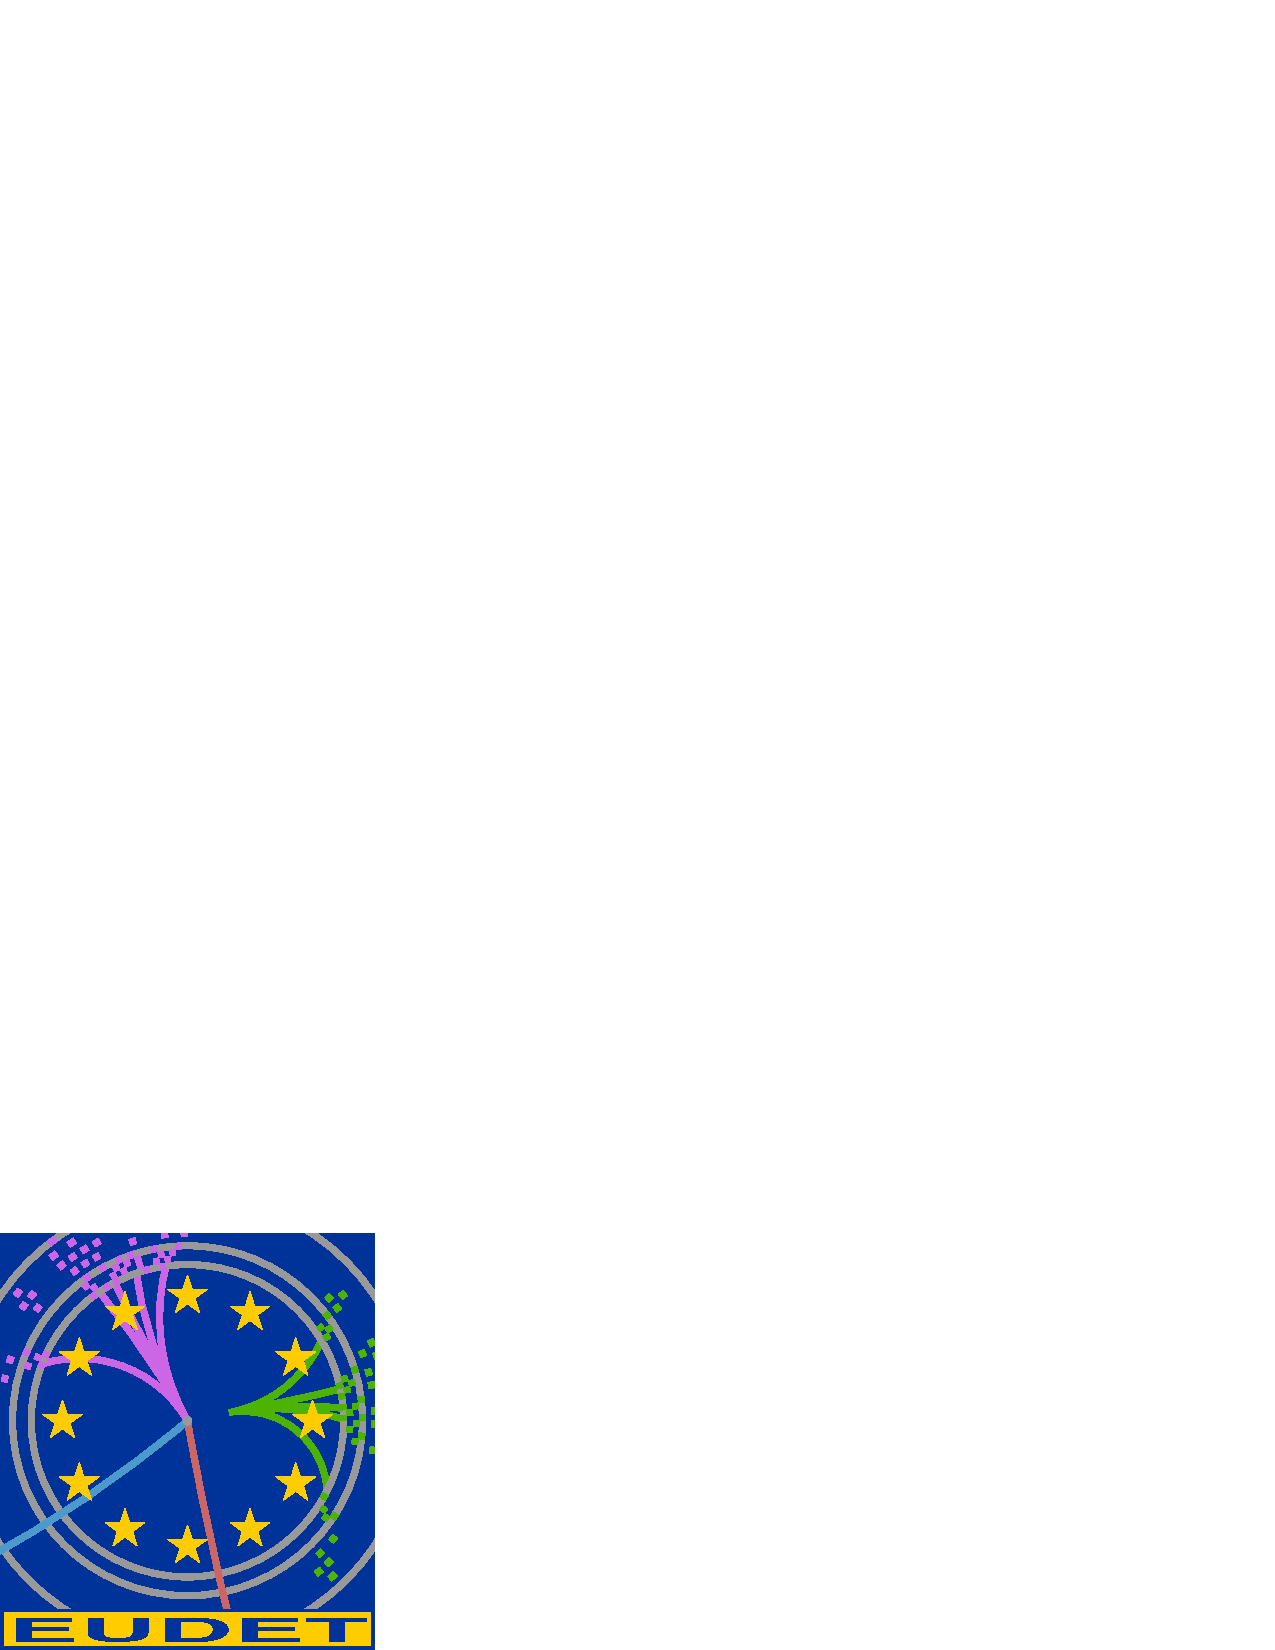
\includegraphics[width=0.1\textwidth]{src/images/logo_eudet} 
\includegraphics[width=0.3\textwidth]{src/images/AIDA_logo_medium} 

\includegraphics[width=0.35\textwidth]{src/images/logo_aida2020}
\vspace{1.5cm}\\
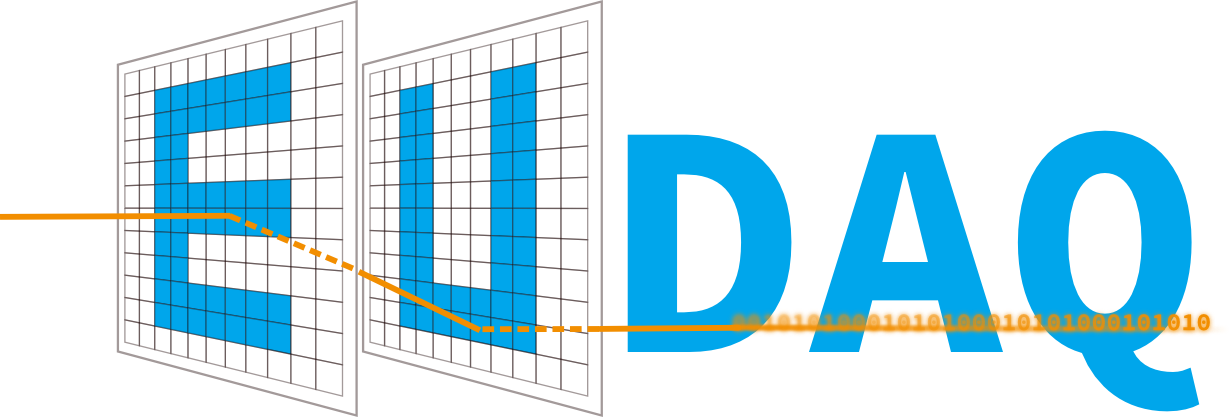
\includegraphics[width=0.7\textwidth]{src/images/eudaq_logo}
\end{center}
}
\title{\Large EUDAQ2 User Manual} 
\author{\normalsize EUDAQ2 Development Team \\
        \normalsize Yi Liu}
%%% CMake uses version.cmake.tex to generate version.cmake.tex within the build/doc/manual/src folder.
\gdef\CMakeLibVersion{v1.4.5*}
 % defines the \CMakeLibVersion command which is
                    % set by CMake to the current EUDAQ version number
                    % (with git hash tag)
\date{\normalsize Last update on September 2017 \\  %\today
for EUDAQ version v2.0.1} %\CMakeLibVersion}

\begin{document}

% Title page
\maketitle
\begin{abstract}
\noindent
This document provides an overview of the EUDAQ software framework,
the data acquisition framework originally developed for use by the
EUDET-type beam telescopes~\cite{telescopesWiki}.
It describes how to install and run the DAQ system and use many of the included utility programs,
and how users may integrate their DAQ systems into the EUDAQ framework
by writing their own: Producer, for integrating the data stream into the acquisition; DataCollector, for merging the muiltple data streams and writing to disk; and DataConverter, for converting data for offline analysis.
\end{abstract}
\newpage

% Contents
% Condense slightly to fit on one page
\begin{spacing}{0.92}
\tableofcontents
\end{spacing}

% Main sections
% !TEX root = EUDAQUserManual.tex
\section{License}
This program is free software: you can redistribute it and/or modify
it under the terms of the Lesser GNU General Public License as published by
the Free Software Foundation, either version 3 of the License, or
(at your option) any later version.

This program is distributed in the hope that it will be useful,
but WITHOUT ANY WARRANTY; without even the implied warranty of
MERCHANTABILITY or FITNESS FOR A PARTICULAR PURPOSE.  See the
Lesser GNU General Public License for more details.
    
You should have received a copy of the Lesser GNU General Public License
along with this program.  If not, see \url{http://www.gnu.org/licenses/}.

% !TEX root = EUDAQUserManual.tex
\section{Introduction}
The EUDAQ software is a data acquisition framework, written in C++,
and designed to be modular and portable, running on Linux, Mac OS X, and Windows.
It was originally written primarily to run the EUDET-type beam telescope~\cite{Roloff:2009zza,Jansen:2016},
but is designed to be generally useful for other systems.

The hardware-specific parts are kept separate from the core,
so that the core library can still be used independently.
For example, hardware-specific parts are two components for the EUDET-type beam telescope: \gls{TLU} and \gls{NI} system for Mimosa 26 sensor read out.

The raw data files generated by the DAQ can be converted to the \gls{LCIO} format,
allowing analysis of the data using the EUTelescope package \cite{eutel2008}.

\subsection{Architecture}
It is split into a number of different processes,
each communicating using TCP/IP sockets (see \autoref{fig:DAQ}).
A central Run Control provides an interface for controlling the whole DAQ system;
other processes connect to the Run Control to receive commands and to report their status.

\begin{figure}[htb]
  \begin{center}
    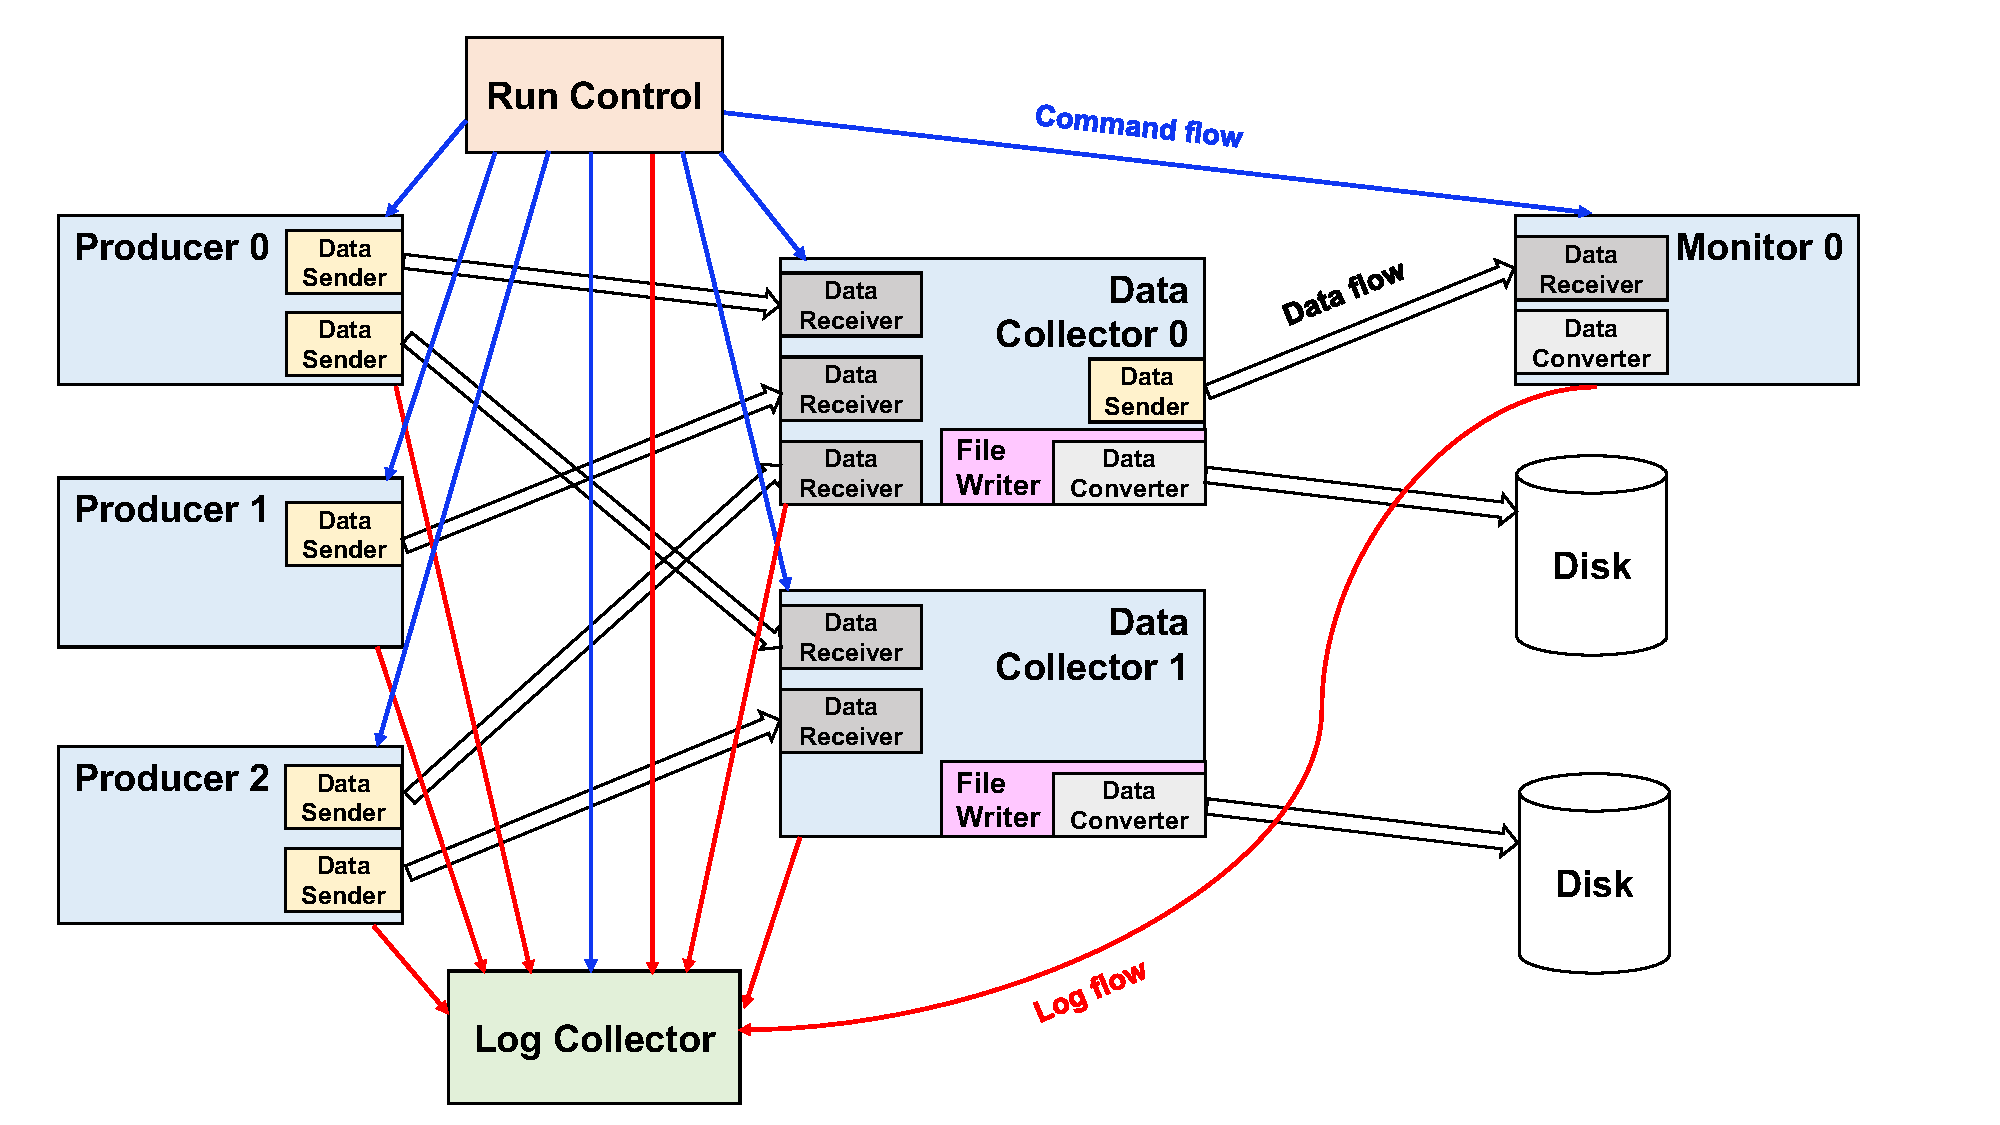
\includegraphics[width=0.9\textwidth]{src/images/eudaq_working_principle}
    \caption{Schematic of the EUDAQ architecture \cite{Spannagel:2016}.}
    \label{fig:DAQ}
  \end{center}
\end{figure}


The DAQ system is made up of a number of different processes that may all be run on the same,
or on different computers. 

\subsubsection{Run Control}
The RunControl is the controller process which manages the full EUDAQ system. There should be always only one instance of RunControl for a runtime setup. All other data taking processes must have the network location of RunControl and anounces themelves to the RunControl. The RunControl takes in the paths of ini/config files and picks up and sends the correlated section to each of the connected processes. As the front end point to users, the RunControl will wait for user input by command line or GUI button click and issue the data taking command to whole EUDAQ system.

\subsubsection{Producer}
Each hardware that produces data will have a Producer process (on the left in \autoref{fig:DAQ}).
This will initialize, configure, stop and start the hardware by receiving the commands from the Run Control (red arrows), read out the data and send it to the Data Collector (blue arrows).

\subsubsection{Data Collector}
The Data Collector is the process that collects all the raw data from the Producers,
merges all the connected incoming streams into a single data stream, and writes it to file.\\

The Data Collector receives all the data streams from all the Producers,
and combines them into a single stream that is written to disk (Storage).
It writes the data in a native raw binary format,
but it can be configured to write in other formats, such as \gls{LCIO}.

\subsubsection{Log Collector}
The Log Collector receives log messages from all other processes (grey arrows),
and displays them to the user, as well as writing them all to file.
This allows for easier debugging, since all log messages are stored together in a central location.

\subsubsection{Monitor}
The Monitor reads the data file and generates online-monitoring plots for display.
In the schematic it is shown to communicate with the Data Collector via a socket,
but it actually just reads the data file from disk.\\

The Online Monitor can be run in one of two modes: online or offline.
In online mode, it connects to the Run Control, so it will know when new runs are started,
and it will automatically open each new data file as it is created.



\subsection{Directory and File Structure}
The EUDAQ software is split into several parts that can each be compiled independently,
and are kept in separate subdirectories.
The general structure is outlined below:

\begin{myitemize}
\item \texttt{main}
  contains the core EUDAQ library with the parts that are common to most of the software,
  and several command-line programs that depend only on this library.
  All definitions in the library should be inside the \texttt{eudaq} namespace.
  It is organized into the following subdirectories:
  \begin{myitemize}
  \item \texttt{main/lib/core}
    contains the source code of the core library,
  \item \texttt{main/lib/lcio}
    contains the source code of the LCIO extension library,
  \item \texttt{main/lib/root}
    contains the source code of the ROOT extension library,
  \item \texttt{main/module}
    contains the source code of the module libraries,
  \item \texttt{main/exe}
    contains the CLI (command line interface) executables source code,
  \end{myitemize}
\item \texttt{gui}
  contains the graphical programs that are built with Qt, such as the RunControl and LogCollector.
\item \texttt{user}
  contains all user provided code shipped with the EUDAQ
  distribution, for example:
  \begin{myitemize}
\item \texttt{user/example}
  contains example code for the integration of user-provided code.
\item \texttt{user/eudet}
  contains the parts that depend on the EUDET-type telescope.
\item e.g. \texttt{user/calice}, \texttt{user/itkstrip}\ldots{}
  contain the code from third-party users.
  \end{myitemize}
\item \texttt{extern}
  global folder which contains external software which themselves are not part of the EUDAQ project.
\item \texttt{cmake}
  global folder which contains cmake files.
\item \texttt{etc}
  contains configuration files of the EUDAQ installation.
\item \texttt{conf}
  contains configuration files for running the beam telescope.
\item \texttt{doc}
  contains source files of the documentation, such as this manual.
\end{myitemize}

Each directory containing code has its own \texttt{src} and \texttt{include} subdirectories,
as well as a local \texttt{CMakeLists.txt} and an optional \texttt{cmake} folder containing the rules
for building that directory using \texttt{CMake}.
Header files have a \texttt{.hh} extension so that they can be automatically recognized as C++,
and source files have either \texttt{.cc} for parts of libraries and \texttt{.cxx} for executables.
In the case of requiring any external dependencies, there could be a local \texttt{extern} folder.

Each directory can contain a \texttt{README.md} file for brief documentation for this specific part, e.g.  
as an installation advice. 
Using the \texttt{*.md} file ending allows the Markdown language \cite{markdownWWW} to be applied. 
Accordingly, the content will be formatted on the the GitHub platform, where the code is hosted online.

\subsection{Executables}
All executable programs from the different subdirectories are in the \texttt{bin} subdirectory. They should all accept a \texttt{-h} (or \texttt{--help}) command-line parameter, which will provide a summary of possible different command-line options.

The executable programs can be split into two different categories: firstly, processes, which are used for the data acquisition and communicating with the Run Control (DAQ); and, secondly, utilities, which are used before or after the data taking in order to access the data files (Test, Development, Tools).
In \autoref{tab:exesall}, an overview of the most important EUDAQ executables is given.

\begin{table}
\centering
\small
\begin{tabular}{ c | l | l | p{4cm}}
  \textbf{Binary} & \textbf{Category} & \textbf{GUI/CLI}  & \textbf{Description}\\
  \hline
  \hline
  \texttt{euRun} & Run Control & GUI & (Sec. \ref{sec:runcontrol}) \\
  \texttt{euLog} & Log Collector & GUI & (Sec. \ref{sec:logcollector}) \\
  \texttt{StdEventMonitor} & legacy Monitor & GUI & \\
  \texttt{euCliRun} & Run Control & CLI & (Sec. \ref{sec:runcontrol}) \\
  \texttt{euCliLogger} & Log Collector & CLI & (Sec. \ref{sec:logcollector}) \\
  \texttt{euCliCollector} & Data Collector & CLI & (Sec. \ref{sec:datacollector}) \\
  \texttt{euCliProducer} & Producer & CLI & (Sec. \ref{sec:testproducer}) \\
  \texttt{euCliMonitor} & Monitor & CLI & (Sec. \ref{sec:onlinemonitor}) \\
  \hline
  \texttt{euCliConverter} & Offline Tool & CLI & data file converter (Sec. \ref{sec:convertafterdatatacking}) \\
  \texttt{euCliReader} & Offline Tool & CLI & dump events from data file (Sec. \ref{sec:dumpafterdatatacking}) \\
  
\end{tabular}
\caption{Overview of EUDAQ executables.}
\label{tab:exesall}
\end{table}


\subsection{Libraries}
The libraries are installed in the \texttt{lib} directory under the install path in Linux/MacOS systems, and to the \texttt{bin} sub-folder in Windows systems. The suffix of libraries name can be \texttt{.so}, \texttt{.dylib}, \texttt{.dll} depending on operate systems. There are 3 category of libraries: core, extension and module: 

\begin{itemize}
\item Core: the core library. It should be always built and installed.
\item Extension: optional features of EUDAQ (e.g.\ support for external data format). Static linked core library.
\item Module: user module. Dynamic load by EUDAQ core library at run-time.
\end{itemize}

In \autoref{tab:liball}, an overview of the all EUDAQ libraries is given.\\

\begin{table}
\centering
\small
\begin{tabular}{ l | l | l | p{4cm}}
  \textbf{Binary} & \textbf{Category} & \textbf{Source Code} & \textbf{Description}\\
  \hline
  \hline
  \texttt{libeudaq\_core} & Core & main$\backslash$lib$\backslash$core & core library \\
  \hline
  \texttt{libeudaq\_lcio} & Extension & main$\backslash$lib$\backslash$lcio & lcio extension library \\
  \texttt{libeudaq\_std} & Extension & main$\backslash$lib$\backslash$std & standard extension library \\
  \hline
  \texttt{libeudaq\_module\_test} & Module & main$\backslash$module$\backslash$test & test module library \\
  \texttt{libeudaq\_module\_example} & Module & user$\backslash$example$\backslash$module &  module library by example user\\
\end{tabular}
\caption{Overview of EUDAQ libraries.}
\label{tab:liball}
\end{table}

% !TEX root = EUDAQUserManual.tex
\section{Installation}
To install the EUDAQ on Linux, Windows or MacOS, you have a choice to download binary distribution package or build it from the source code.

\subsection{Binary Package Installation}
The portable precompiled packages are avaliable from EUDAQ website. You could unpack the installation package to any folder and run the example directly. Please note, not all features of EUDAQ are enabled in the precompiled package, since it is not sure at compiling time whether the end user have the necessary dependency package installed.

\subsection{Building from Source Code}

The installation is described in four steps:%
\footnote{Quick installation instructions are also described on \url{http://eudaq.github.io/} or in the main \texttt{README.md} file of each branch, e.g. \url{https://github.com/eudaq/eudaq/blob/master/README.md}.}
\begin{enumerate}
\item Installation of (required) prerequisites
\item Downloading the source code (GitHub)
\item Configuration of the code (CMake)
\item Compilation of the code
\end{enumerate}

If problems occur during the installation process, please have a look at the issue tracker on GitHub.%
\footnote{Go to \url{https://github.com/eudaq/eudaq/issues}} 
Here you can search whether your problem had already been experienced by someone else, or you can open a new issue (see \autoref{sec:reporting}).

\subsubsection{Prerequisites}

EUDAQ has some dependencies on other software, but some features do rely on other packages:
\begin{itemize}
\item To get the code and stay updated with the central repository on GitHub, git is used.
\item To configure the EUDAQ build process, the CMake cross-platform, open-source build system is used.
\item To compile EUDAQ from source code requires a compiler that implements the C++11 standard.
\item Qt is required to build GUIs of e.g.\ the RunControl or LogCollector. 
\item ROOT is required for the lagecy StdEventMonitor.
\end{itemize}

\paragraph{Git}
Git is a free and open source distributed version control and is available for all of the usual platforms \cite{gitWWW}. 
It allows local version control and provides repositories, but also enables communication with central online repositories like GitHub.
   
In order to get the EUDAQ code and stay updated with the central repository on GitHub, git is used (see \autoref{sec:downloadingEUDAQ}).
For EUDAQ code development, requiring different versions (tags) or branches (development repositories), git is also used. %%%% (see \autoref{sec:contributing}).


\paragraph{CMake (required)}
In order to generate configuration files for building EUDAQ (makefiles) independently from the compiler and the operating platform, the CMake (at least version 3.1) build system is used.

CMake is available for all major operating systems from \url{http://www.cmake.org/cmake/resources/software.html}. 
On most Linux distributions, it can usually be installed via the built-in package manager (aptitude/apt-get/yum etc.) and on MacOS using packages provided by e.g. the MacPorts or Fink projects.

\paragraph{C++11 compliant compiler (required)}
The compilation of the EUDAQ source code requires a C++11 compliant compiler and has been tested with GCC (at least version 4.8.1), Clang (at least version 3.1), and MSVC (Visual Studio 2013 and later) on Linux, OS X and Windows.

\paragraph{Qt (for GUI)}
The graphical interface of EUDAQ uses the Qt graphical framework.
In order to compile the \texttt{gui} subdirectory, you must therefore have Qt installed.
It is available in most Linux distributions as the package \texttt{qt5-devel} or \texttt{qt5-dev}.
It can also be downloaded and installed from \url{http://download.qt.io/archive/qt/}. 

\paragraph{ROOT (for the StdEventMonitor)}
\label{sec:Root}
%%%% To enable the EUDAQ extensions library support to ROOT, EUDAQ needs to be compiled and linked to the ROOT library.
The Online Monitor uses the ROOT package.
It can be downloaded from \url{http://root.cern.ch}.

Make sure ROOT's \texttt{bin} subdirectory is in your path, so that the \texttt{root-config} utility can be run.
This can be done by sourcing the \texttt{thisroot.sh} (or \texttt{thisroot.ch} for csh-like shells)
script in the \texttt{bin} directory of the ROOT installation:
\begin{listing}[mybash]
source /path-to/root/bin/thisroot.sh
\end{listing}

\paragraph{LCIO (for LCIO extension)}
\label{sec:LCIO}
To enable the writing of \gls{LCIO} files, or the conversion of native files to \gls{LCIO} format,
EUDAQ must be linked against the \gls{LCIO} libraries.
When the LCIO option is enabled during the configuration step, source files will be download from the internet and compiled automatically.

%%%%%%%%%%%%%%%%%%%%%%%%%%%%%%%%%%%%%%%%%%%%%%%%%%%%%%%%%%%
\subsubsection{Obtaining the source code}
\label{sec:downloadingEUDAQ}

The EUDAQ source code is hosted on GitHub \cite{githubEUDAQ}. 
Here, we describe how to get the code and install a stable version release. 
In order to get information about the work flow of developing EUDAQ code, please find the relevant information in see \autoref{sec:contributing}.

\paragraph{Downloading the code (clone)}
We recommend using git to download the software,
since this will allow you to easily update to newer versions.
The source code can be downloaded with the following command:
\begin{listing}[mybash]
git clone https://github.com/eudaq/eudaq.git eudaq
\end{listing}
This will create the directory \texttt{eudaq}, and download the latest
version into it. 

\textit{Note:} Alternatively and without version control, you can also download a zip/tar.gz file of EUDAQ releases (tags) from \url{https://github.com/eudaq/eudaq/releases}. 
By downloading the code, you can skip the next two subsections. 

\paragraph{Changing to a release version (checkout)}
After cloning the code from GitHub, your local EUDAQ version is on the master branch (check with \texttt{git status}).  
For using EUDAQ without development or for production environments (e.g. at test beams), we strongly recommend to use the latest release version. 
Use 
\begin{listing}[mybash]
git tag 
\end{listing}
in the repository to find the newest stable version as the last entry.
In order to change to this version in your local repository, execute e.g. 
\begin{listing}[mybash]
git checkout v2.0.0alpha
\end{listing}
to change to version v2.0.0alpha.

\paragraph{Updating the code (fetch)}
If you want to update your local code, e.g to get the newest release versions, execute in the \texttt{eudaq} directory: 
\begin{listing}[mybash]
git fetch
\end{listing}
and check for new versions with \texttt{git tag}. 


\subsubsection{Configuration via CMake}
\label{sec:cmake}
CMake supports out-of-source configurations and generates building files for compilation (makefiles). 
Enter the \texttt{build} directory and run CMake, i.e.
\begin{listing}[mybash]
cd build
cmake ..
\end{listing}
CMake automatically searches for required packages and verifies that all dependencies are met using the \texttt{CMakeLists.txt} scripts in the main folder and in all sub directories. 

You can modify this default behavior by passing the \texttt{-D[eudaq\_build\_option]} option to
CMake where \texttt{[name]} refers to an optional component, e.g.
\begin{listing}[mybash]
cmake -DEUDAQ_BUILD_GUI=ON  ..
\end{listing}
to disable the GUI but enable additionally executable of the TLU producer.
The most important building options are given in \autoref{tab:cmakeoptions}.

If you are not familiar with cmake, cmake-gui is nice GUI tool to help you configure the project.

\begin{table}[!h]
{\footnotesize
\begin{tabular}{l|l|p{2cm}|p{5.5cm}}
option &  default &  dependency & comment \\
\hline
\texttt{EUDAQ\_BUILD\_EXECUTABLE} &  \texttt{<auto>} & none & Builds main EUDAQ executables.\\
\texttt{EUDAQ\_BUILD\_GUI} & \texttt{<auto>} & Qt5 & Builds GUI executables, such as the RunControl (euRun) and LogCollector (euLog).\\
\texttt{EUDAQ\_BUILD\_MANUAL} & \texttt{OFF} & LaTex &  Builds manual in pdf-format.  \\
%% \texttt{EUDAQ\_BUILD\_NREADER} & \texttt{OFF} & EUTelescope, LCIO &  Builds native reader Marlin processor used for data conversion into LCIO.\\
\texttt{EUDAQ\_BUILD\_STDEVENT\_MONITOR} & \texttt{auto} & ROOT6 &  Builds lagecy standardevent monitor.  \\
\texttt{EUDAQ\_INSTALL\_PREFIX} & \texttt{<source\_folder>} & none & In order to install the executables into \texttt{bin} and the library into \texttt{lib} of a specific path, instead of into the \texttt{<source\_folder>} path.\\
\texttt{EUDAQ\_LIBRARY\_BUILD\_CLI} & \texttt{ON} & none & Builds extension library of command line interface.\\
\texttt{EUDAQ\_LIBRARY\_BUILD\_LCIO} & \texttt{<auto>} & LCIO & Builds LCIO extension library.\\
%% \texttt{EUDAQ\_LIBRARY\_BUILD\_ROOT} & \texttt{<auto>} & ROOT & Builds ROOT extension library.\\
\texttt{EUDAQ\_LIBRARY\_BUILD\_TEST} & \texttt{ON} & none & Builds extension library for develop test.\\
\texttt{USER\_EXAMPLE\_BUILD} & \texttt{ON} & none & Builds example user code.\\
\texttt{USER\_\{user\_name\}\_BUILD} & \texttt{<unknown>} & \texttt{<unknown>} & Builds user code inside user folder \{user\_name\}.\\
\texttt{CMAKE\_BUILD\_TYPE} & \texttt{RelWithDebInfo} & \texttt{none} & Only affect the building on Linux/MacOS, see CMake manual.\\
\end{tabular}
\caption{Options for CMake.}
\label{tab:cmakeoptions}
}
\end{table}

\textit{Note:} After building files by running \texttt{cmake ..}, you can list all possible options and their status by running \texttt{cmake -L}. 
Using a GUI version of CMake shows also all of the possible options.   

Corresponding settings are cached, thus they will be used again next time CMake is run.
If you encounter a problem during installation, it is recommended to clean the cache by just removing all files from the build folder, since it only contains automatically generated files. 


%%%%%%%%%%%%%%%%%%%%%%%%%%%%%%%%%%%%%%%%%%%%%%%%%%%%%%%%%%%%%%%55
\subsubsection{Compilation}
Universal command for all systems:
\begin{listing}[mybash]
cmake --build {source_folder}/build --target install
\end{listing}

Done!

% !TEX root = EUDAQUserManual.tex
\section{Run an Example Setup}
This section will describe running the DAQ system, mainly from the point of view of running an example setup as a demonstration without dedicated hardware.
However, this description can be applied to a detector DAQ system in general.

\subsection{Target Setup}
In this example, a user hardware device is simulated and implemented as an example Producer which can be configured to generate fake data. This works similarly to a real Producer, but does not talk to any real hardware. An example DataCollector is also implemented. \\
The runtime setup consists of the following EUDAQ processes.
\begin{description}
\ttitem{RunControl}
an example RunControl instanced by GUI application.
\ttitem{LogCollector}
a default LogCollector instanced by GUI application.
\ttitem{Producer}
Two example Producers instanced by the CLI command. Both of them produces events at a rate of 1\,Hz, they may have time offset of start run.
\ttitem{DataCollector}
an example DataCollectors instanced by the CLI command.
\ttitem{Monitor}
an example monitor which prints out the asambled Event from the DataCollector in the command line terminal.
\end{description}

\subsection{Preparation}
Some preparation is needed to make sure the environment is set up correctly and
the necessary TCP ports are not blocked before the DAQ can run properly.

\subsubsection{Directories}
If no specified path is passed to EUDAQ (by configuration file or command line parameter), EUDAQ will assume the working folder where executable is started up is writable. Data and log files will be stored in the working folder.

\subsubsection{Init/Config-Files}\label{sec:ConfigFiles}
\texttt{$\ast$.ini}-files for initialization and \texttt{$\ast$.conf}-files for configuration
are text files in a specific format, containing name-value pairs separated into different sections.\footnote{\url{https://en.wikipedia.org/wiki/INI\_file}}
Any text from a \texttt{\#} character until the end of the line is treated as a comment, and
ignored.  
Each section in the config file is delimited by a pair of names seperated by a perioid in square brackets (e.g. \verb@[Producer.Example]@).
The name before peroid represents the type of process to which it applies, the one after peroid is the runtime name of the applied process.
. There is an exception, the section for Run Control is always \verb@[RunControl]@ in which there is no runtime name. 
Within each section, any number of parameters may be specified,
in the form \mbox{\texttt{Name = Value}}.  The EUDAQ native supported parmaters have a common prefix \texttt{EUDAQ\_}.
It is then up to the individual processes how these parameters are interpreted.

During the initialization and configuration, each process gets its section and does not know about the other parts of the ini/conf files.
\myinputlisting[conf]{-30}{user/example/misc/Ex0.ini}

\myinputlisting[conf]{-30}{user/example/misc/Ex0.conf}

\subsubsection{Ports and Firewall}
The different processes communicate between themselves using TCP/IP sockets. The ports can be configured when calling the the processors on the command line (see below). By default, TCP port 44000 is listened to by the RunControl, and TCP port 44002 is listened to by the LogCollector to get connections from clients. The DataCollector will pick a random TCP port to listen to and get incoming data from its connected Producers if there is no specific port assigned explicitly by user.

When all EUDAQ processes run on the same computer, common firewalls will not affect the TCP connections among them. However, running EUDAQ distributively on several computers may have issue from firewall blocking. You will have to open up those TCP ports for incoming connections, temporally shut down the firewall. Shutting down the firewall is operating-system dependent.\\

In this example, all processes will run on the same Linux computer, so we can skip the setup of TCP port.

%%%%%%%%%%%%%%%%%%%%%%%%%%%%%%%%%%%%%%%%%%%%%%%%%%%%%%%%%%%%%%%55
\subsection{Startup}
To start EUDAQ, all of the necessary processes have to be started in the correct order.
The first process must be the Run Control,
since all other processes will attempt to connect to it when they start up.
Then it is recommended to start the Log Collector,
since any log messages it receives may be useful
to help with debugging in case everything does not start as expected.
Finally, the Data Collector, Producers and Monitor can be started in any order you want.

\subsubsection{RunControl}
\label{sec:runcontrol}
There are two versions of the RunControl -- a text-based version \texttt{euCliRun} and a graphical version \texttt{euRun} (see \autoref{fig:RunControl}).

The command line pattern to start up a Log Collector is:
\begin{listing}[mybash]
$[euRun]$ -n {code_name} -a tcp://{listening_port}
\end{listing}

\begin{description}
\ttitem{-n \param{code\_name}}
optional, if it is not specified, default RunControl will be instanced. 
\ttitem{-a \param{listening\_addr}}
optional, \texttt{listening\_port} default value is 44000.
\end{description}

For this example setup, we will startup the euRun GUI which internally instances the default Run Control and make it serve at TCP port 44000:\\
\begin{listing}[mybash]
$[euRun]$ -n Ex0RunControl -a tcp://44000
\end{listing}

After executing the above command, a new GUI windows is shown in \autoref{fig:RunControl}.
\begin{figure}[htb]
  \begin{center}
    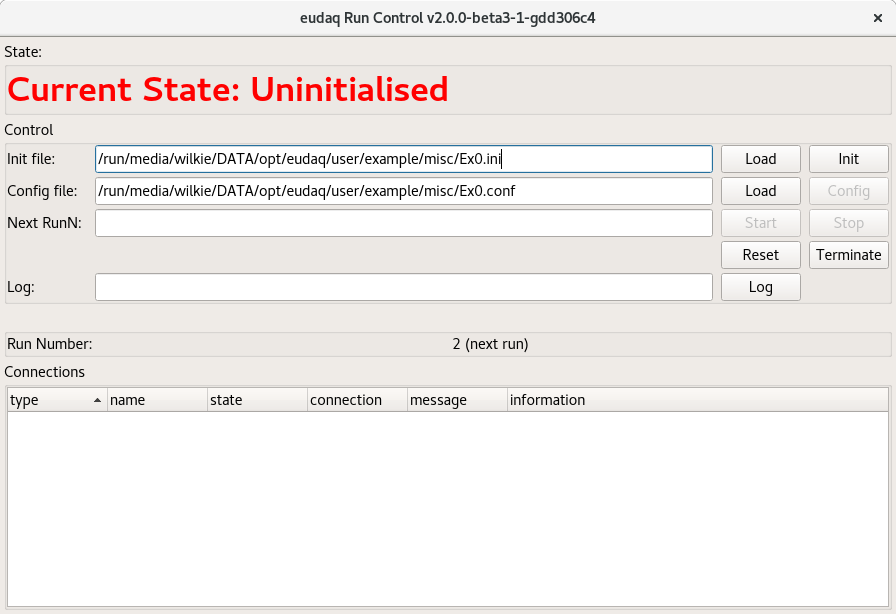
\includegraphics[width=0.8\textwidth]{src/images/eurun_ui}
    \caption{The Run Control graphical user interface.}
    \label{fig:RunControl}
  \end{center}
\end{figure}

\paragraph{Initialization Section}
\begin{listing}[conf]
[RunControl]
# The Ex0RunControl does not need any paramters.
\end{listing}

\paragraph{Configuration Section}
\begin{listing}[conf]
[RunControl]
EX0_STOP_RUN_AFTER_N_SECONDS = 60
\end{listing}

\subsubsection{LogCollector}
\label{sec:logcollector}
It is recommended to start the Log Collector directly after having started the Run Control and before starting other processors in order to collect all log messages generated by all other processes.

There are also two versions of the Log Collector.
The graphical version is called \texttt{euLog},
and the text-based version is called \texttt{euCliLogger}.

The command line pattern to startup a Log Collector is:
\begin{listing}[mybash]
$[euLog]$ -r tcp://{run_contorl_hostname}:{run_contorl_port} -a tcp://{listening_port}
\end{listing}

\begin{description}
\ttitem{-r \param{runcontrol\_addr}}
optional, \texttt{run\_control\_hostname} default value: localhost;  \texttt{run\_contorl\_port}  default value: 44000.
\ttitem{-a \param{listening\_addr}}
optional, \texttt{listening\_port} default value is 44002.
\end{description}

For this example setup, we will startup the GUI version of Log Collector, connect it to the Run Contorl at local port 44000 and make it serve at TCP port 44002:\\
\begin{listing}[mybash]
$[euLog]$ -r tcp://localhost:44000 -a tcp://44002
\end{listing}

After executing the above command, a new GUI window, as shown in \autoref{fig:LogCollector}, is opened and the RunControl displays a new connection, as seen in \autoref{fig:RunControl_con_log}.
\begin{figure}[htb]
  \begin{center}
    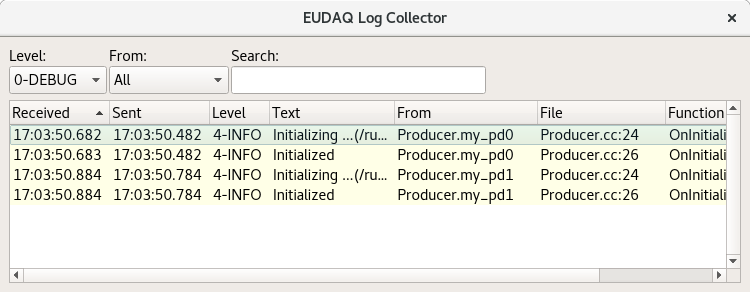
\includegraphics[width=\textwidth]{src/images/eulog_ui}
    \caption{The Log Collector graphical user interface.}
    \label{fig:LogCollector}
  \end{center}
\end{figure}


\paragraph{Initialization Section}
\begin{listing}[conf]
[LogCollector.log]
# Currently, all LogCollectors have a hardcoded runtime name: log
EULOG_GUI_LOG_FILE_PATTERN = myexample_$12D.log
# the $12D will be converted a data/time string with 12 digits. 
# the file path is allowed add as prefix in this file name pattern,
# otherwise the log file is saved in working folder.
\end{listing}

\paragraph{Configuration Section}
\begin{listing}[conf]
[LogCollector.log]
# Currently, all LogCollectors have a hardcoded runtime name: log
# nothing
\end{listing}

\subsubsection{DataCollector}
\label{sec:datacollector}
There is only a text-based version called \texttt{euCliCollector}.
The command line pattern to startup a DataCollector is:
\begin{listing}[mybash]
$[euCliCollector]$ -n {code_name} -t {runtime_name} -r tcp://{run_control_hostname}:{run_contorl_port} -a tcp://{listening_port}
\end{listing}

\begin{description}
\ttitem{-n \param{code\_name}}
required.
\ttitem{-t \param{runtime\_name}}
required.
\ttitem{-r \param{runcontrol\_addr}}
optional, \texttt{run\_control\_hostname} default value: localhost;  \texttt{run\_contorl\_port}  default value: 44000.
\ttitem{-a \param{listening\_addr}}
optional, \texttt{listening\_port} default value is random.
\end{description}

By default, an example DataCollector \texttt{Ex0TgDataCollector} is available with the standard installation of EUDAQ.
For this example setup, we will startup two instances of \texttt{Ex0TsDataCollector} with runtime names \texttt{my\_dc} and \texttt{another\_dc}\\
\begin{listing}[mybash]
$[euCliCollector]$ -n Ex0TgDataCollector -t my_dc -r tcp://localhost:44000 -a tcp://45001
\end{listing}

\paragraph{Initialization Section}
\begin{listing}[conf]
[DataCollector.my_dc]
# nothing
\end{listing}

\paragraph{Configuration Section}
\begin{listing}[conf]
[DataCollector.my_dc]
EUDAQ_MN=my_mon
# send assambled event to the monitor with runtime name my_mon;
EUDAQ_FW=native
# the format of data file
EUDAQ_FW_PATTERN=$12D_run$6R$X
# the name pattern of data file
# the $12D will be converted a data/time string with 12 digits.
# the $6R will be converted a run number string with 6 digits.
# the $X will be converted the suffix name of data file.
# the file path is allowed add as a prefix to this name pattern,
# otherwise the data file is saved in working folder.
\end{listing}

\subsubsection{Producer}
\label{sec:testproducer}
There is only a text-based version called \texttt{euCliProducer}.
The command line pattern to startup a Producer is:
\begin{listing}[mybash]
$[euCliProducer]$ -n {code_name} -t {runtime_name} -r tcp://{run_control_hostname}:{run_contorl_port}
\end{listing}

\begin{description}
\ttitem{-n \param{code\_name}}
required.
\ttitem{-t \param{runtime\_name}}
required.
\ttitem{-r \param{runcontrol\_addr}}
optional, \texttt{run\_control\_hostname} default value: localhost;  \texttt{run\_contorl\_port}  default value: 44000.
\end{description}

By default, an example Producer \texttt{Ex0Producer} is available with the standard installation of EUDAQ.
For this example setup, we will startup two instances of \texttt{Ex0Producer} with runtime names \texttt{my\_pd0} and \texttt{my\_pd0}\\
\begin{listing}[mybash]
$[euCliProducer]$ -n Ex0Producer -t my_pd0 -r tcp://localhost:44000
$[euCliProducer]$ -n Ex0Producer -t my_pd1 -r tcp://localhost:44000
\end{listing}

\paragraph{Initialization Section}
\begin{listing}[conf]
[Producer.my_pd0]
EX0_DEV_LOCK_PATH = /tmp/mydev0.lock

[Producer.my_pd1]
EX0_DEV_LOCK_PATH = /tmp/mydev1.lock
\end{listing}

\paragraph{Configuration Section}
\begin{listing}[conf]
[Producer.my_pd0]
EUDAQ_DC=my_dc
# send events to the producer with runtime name my_dc.
# it is allowed to have a configure line as "EUDAQ_DC=his_dc,her_dc"
# to make the producer send events to muiltiple DataCollectors.  
EX0_PLANE_ID=0
EX0_DURATION_BUSY_MS=1
EX0_ENABLE_TRIGERNUMBER=1

[Producer.my_pd1]
EUDAQ_DC=my_dc
# send events to the producer with runtime name my_dc.
EX0_PLANE_ID=1
EX0_DURATION_BUSY_MS=1
EX0_ENABLE_TRIGERNUMBER=1
\end{listing}

\subsubsection{Monitor}
\label{sec:onlinemonitor}
There is a text-based version called \texttt{euCliMonitor}.
The command line pattern is:
\begin{listing}[mybash]
$[euCliMonitor]$ -n {code_name} -t {runtime_name} -r tcp://{run_control_hostname}:{run_contorl_port} -a tcp://{listening_port}
\end{listing}
\begin{description}
\ttitem{-n \param{code\_name}}
required.
\ttitem{-t \param{runtime\_name}}
required.
\ttitem{-r \param{runcontrol\_addr}}
optional, \texttt{run\_control\_hostname} default value: localhost;  \texttt{run\_contorl\_port}  default value: 44000.
\ttitem{-a \param{listening\_addr}}
optional, \texttt{listening\_port} default value is random.
\end{description}

By default, an example Monitor \texttt{Ex0Monitor} is available with the standard installation of EUDAQ. To simplify this example, the \texttt{Ex0Monitor} has no graphic windows, it can only print Event in commnad line terminal.
For this example setup, we will startup two instances of \texttt{Ex0Producer} with runtime names \texttt{my\_mon}\\
\begin{listing}[mybash]
$[euCliMonitor]$ -n Ex0Monitor -t my_mon -r tcp://localhost:44000 -a tcp://45002
\end{listing}

\paragraph{Initialization Section}
\begin{listing}[conf]
[Monitor.my_mon]
# nothing
\end{listing}

\paragraph{Configuration Section}
\begin{listing}[conf]
[Monitor.my_mon]
EX0_ENABLE_PRINT=0
EX0_ENABLE_STD_PRINT=0
EX0_ENABLE_STD_CONVERTER=1
\end{listing}

\subsection{Operating}
Once all the processes have been started, the RunControl GUI window will be as in \autoref{fig:RunControl_operate}.
\begin{figure}[htb]
  \begin{center}
    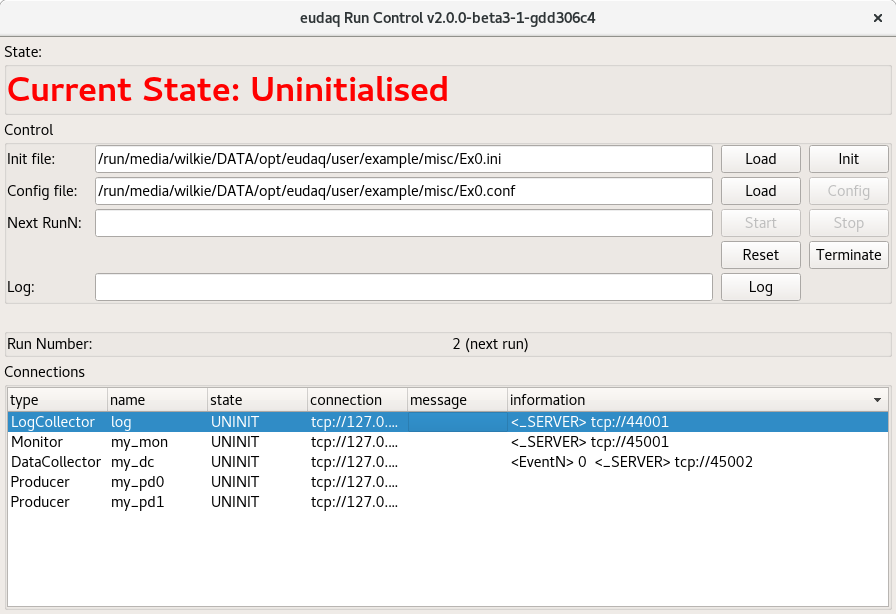
\includegraphics[width=0.8\textwidth]{src/images/eurun_ui_connected}
    \caption{The RunControl with all connections of the example setup.}
    \label{fig:RunControl_operate}
  \end{center}
\end{figure}

All of the processes report their status to the RunControl.
Depending on their status, EUDAQ and all processes can be initialized, configured or re-configured, data taking (runs) can be started and stopped, and the software can be terminated.

\begin{itemize}
\item First, the appropriate initialization file should be selected (see \autoref{sec:ConfigFiles} for creating and editing init-files). Then the \texttt{Init} button can be pressed,
which will send an initialization command to all connected processes.

\item Second, the appropriate configuration should be selected 
  (see \autoref{sec:ConfigFiles} for creating and editing configurations).
Then the \texttt{Config} button can be pressed,
which will send a configuration command
(with the contents of the selected configuration file) to all connected processes.
so that this information is always available along with the data.
\item Once all connected processes are fully configured, a run may be started, by pressing the \texttt{Start} button.
Whatever text is in the corresponding text box (``\texttt{Run:}'') when the button is pressed
will be stored as a comment in the data file.
This can be used to help identify the different runs later.
\item Once a run is completed, it may be stopped by pressing the \texttt{Stop} button.
\item At any time, a message may be sent to the log file by filling in the (``\texttt{Log:}'') text box and pressing the corresponding button.
The text should appear in the LogCollector window, and will be stored in the log file for later access.
\item Once the run is stopped, the system may be reconfigured with a different configuration, or another run may be started; or EUDAQ can be terminated.
  
\end{itemize}


\subsection{After data taking}
By default, EUDAQ provides tools to manage the the data saved in file by native EUDAQ format. Those tools could also be examples for users to write new code for more specific purpose. 
\subsubsection{Dump data}
\label{sec:dumpafterdatatacking}
To dump print Event from data file, the tool \texttt{euCliReader} is provided. The command line pattern is:
The command line pattern is:
\begin{listing}[mybash]
$[euCliReader]$ -i {input_file} -e {event_number_begin} -E {event_number_end} -tg {trigger_number_begin} -TG {tigger_number_end} -ts {timestamp_begin} -TS {timestamp_end} -s -std
\end{listing}
\begin{description}
\ttitem{-i \param{input\_file}}
required, the path of the input data file
\ttitem{-e \param{event\_number\_begin}}
optional, the low limit of event number to be printed 
\ttitem{-E \param{event\_number\_end}}
optional, the high limit of event number to be printed 
\ttitem{-tg \param{trigger\_number\_begin}}
optional, the low limit of trigger number to be printed 
\ttitem{-TG \param{trigger\_number\_end}}
optional, the high limit of trigger number to be printed 
\ttitem{-ts \param{timestamp\_begin}}
optional, the low limit of timestamp to be printed 
\ttitem{-TS \param{timestamp\_end}}
optional, the high limit of timestamp to be printed
\ttitem{-s}
optional, enable the print of statistics 
\ttitem{-std}
optional, enable the Standard Event Converter and print out StdEvent
\end{description}

The option pairs \texttt{-e -E}, \texttt{-tg -TG} and \texttt{-ts -TS} apply range limites and pick up the most intreasting Event from data file. If an option pair is not specified by user, there will be not range limit for this option pair.

\subsubsection{Convert data format}
\label{sec:convertafterdatatacking}
To convert Event from data file, the tool \texttt{euCliConverter} is provided. The command line pattern is:
The command line pattern is:
\begin{listing}[mybash]
$[euCliConverter]$ -i {input_file} -o {output_file} -ip
\end{listing}
\begin{description}
\ttitem{-i \param{input\_file}}
required, the path of the input data file
\ttitem{-o \param{output\_file}}
required, the path of the output data file. 
\ttitem{-ip}
optional, enable the print of input Event 
\end{description}

If the output file has the suffix \texttt{slcio} and LCIO feature of EUDAQ is enabled at compiling time, it will generate LCIO data file.

% !TEX root = EUDAQUserManual.tex
\section{Integration with User Hardware}\label{sec:Integration}
EUDAQ itself is only a data taking framework. It means that the users with their dedicated hardware and readout software are required to write some code to bridge the hardware specific readout software to the EUDAQ framework. The minimum adaptation task is to write a Producer for each piece of hardware, a Data Collector to receive the data (a.k.a.\ Event) from the Producers. 

\subsection{Announcement of Derived Class}
The derived EUDAQ classes provided by the user will be compiled and packed to a dynamic shared library (EUDAQ Module Library). At compiling/linking time of EUDAQ core library, it does not know of the existence of any Module Library. When the EUDAQ core library is being loaded by any application, the core library will look for any library file with the name prefix libeudaq\_module\_ in the module folder. All pattern matched libraries will be loaded. It is the point at which each derived EUDAQ class announces itself to the EUDAQ runtime environment.

Technically, the announcement of a derived class is done by a call to the correlated static function provided by a generic C++ template (eudaq::Factory). \autoref{tab:derivable} is the list of derivable EUDAQ classes.

\begin{table}
\centering
\small
\begin{tabular}{ l | l }
  \textbf{Class} & \textbf{Description}\\
  \hline
  \texttt{eudaq::Producer} & Sec. \ref{sec:ProducerWriting}\\
  \texttt{eudaq::DataCollector} & Sec. \ref{sec:DataCollectorWriting}\\
  \texttt{eudaq::RunControl} & Sec. \ref{sec:RunControlWriting}\\
  \texttt{eudaq::Event} &  Sec. \ref{sec:Event} \\
  \texttt{eudaq::LogCollector} & Sec. \ref{sec:logcollector} \\
  \texttt{eudaq::Monitor} & Sec. \ref{sec:MonitorWriting}\\
  \texttt{eudaq::FileWriter} & Sec. \ref{sec:FileWriterWriting}\\
  \texttt{eudaq::FileReader} & Sec. \ref{sec:FileReaderWriting}\\
  \texttt{eudaq::StdEventConverter} & Sec. \ref{sec:DataConverter} \\
  \texttt{eudaq::LCEventConverter} & Sec. \ref{sec:DataConverter} \\
  \texttt{eudaq::TransportServer} & internal only \\
  \texttt{eudaq::TransportClient} & internal only \\
\end{tabular}
\caption{Derivable Classes.}
\label{tab:derivable}
\end{table}

\subsection{Serializable}
As a distributed DAQ framework, a runtime setup of the EUDAQ system include several applications. Data objects will go through the boundary of an application or a computer. Those data objects should have the capability to be serialized. When a data object is serialized, all the crucial data of this data object is fed to serialized memory which then can be sent by plain binary to another application and reconstructed as a copy of the original data object. \\

All the classes which hold serializable data are derived from a base serializable class (eudaq::Serializable). All serializable data class
should implement the function \texttt{Serialize} which serializes the inner data object and feeds an eudaq::Serializer, and a constructor function which takes the reference of eudaq::Deserializer as input parameter.\\

\autoref{tab:serializable} is the list of serializable EUDAQ classes.

\begin{table}
\centering
\small
\begin{tabular}{ l | l }
  \textbf{Class} & \textbf{Description}\\
  \hline
  \texttt{eudaq::Event} & Sec. \ref{sec:Event} \\
  \texttt{eudaq::Configuration} & Contains configuration information \\
  \texttt{eudaq::LogMessage} & Messages reported to the LogCollector \\
  \texttt{eudaq::Status} & States reported to the RunControl \\
\end{tabular}
\caption{Serializable Classes.}
\label{tab:serializable}
\end{table}

\subsubsection{Event}\label{sec:Event}
eudaq::Event is most important serializable class which holds physics data from the hardware. The Producer is the EUDAQ component which creates the object eudaq::Event and feeds it the physics data from measurements.  \autoref{tab:eventdata} lists the variables inside the eudaq::Event. \\

\begin{table}
\centering
\small
\begin{tabular}{ l | l | l }
  \textbf{variable} & \textbf{C++ type} & \textbf{Description}\\
  \hline
  \texttt{m\_type} & \texttt{uint32\_t} & event type\\
  \texttt{m\_version} & \texttt{uint32\_t} & version\\
  \texttt{m\_flags} & \texttt{uint32\_t} & flags\\
  \texttt{m\_stm\_n} & \texttt{uint32\_t} & device/stream number\\
  \texttt{m\_run\_n} & \texttt{uint32\_t} & run number\\
  \texttt{m\_ev\_n} & \texttt{uint32\_t} & event number\\
  \texttt{m\_tg\_n} & \texttt{uint32\_t} & trigger number\\
  \texttt{m\_extend} & \texttt{uint32\_t} & reserved word\\
  \texttt{m\_ts\_begin} & \texttt{uint64\_t} & timestamp at the begin of event\\
  \texttt{m\_ts\_end} & \texttt{uint64\_t} & timestamp at the end of event\\
  \texttt{m\_dspt} & \texttt{std::string} & description\\
  \texttt{m\_tags} & \texttt{std::map<std::string, std::string>} & tags\\
  \texttt{m\_blocks} & \texttt{std::map<uint32\_t, std::vector<uint8\_t>>} & blocks of raw data\\
  \texttt{m\_sub\_events} & \texttt{std::vector<EventSPC>} & pointers of sub events\\
\end{tabular}
\caption{Variables of eudaq::Event.}
\label{tab:eventdata}
\end{table}

The \texttt{m\_blocks} is physics data which can only be known by the user who owns the hardware. There is a pair of timestamps to define the time slice when the physics event occurs, and a trigger number to identify the trigger sequence. Timestamps and trigger number are optional to be set if you are going to use them to synchronize data from multiple stream/device. It is also possible to have sub events inside an eudaq::Event object. The sub eudaq::Event objects are held by std::shared\_ptr, see the next section.

\subsection{Ownership}
std::shared\_ptr and std::unique\_ptr are heavily used in EUDAQ to hold the object pointers of the serializable class and the derivable class.  They get rid of the unnecessary and ineffective memory copy and are exception safe for any memory leakage.

\subsection{Command/Status Handling}
\subsubsection{RunControl and CommandReceiver}\label{sec:runcontrol}
\paragraph{RunControl} eudaq::RunControl is the command sender which issues commands according to user actions from the GUI or CLI.
\paragraph{CommandReceiver} eudaq::Producer, eudaq::DataCollector, eudaq::LogCollector and eudaq::Monitor are command receivers (eudaq::CommandReceiver) which executes the correlated function according to the command. The command receiver will set up a status (eudaq::Status) and report the status to RunControl.

\subsubsection{State Model}\label{sec:fsm}
\begin{figure}
\begin{center}
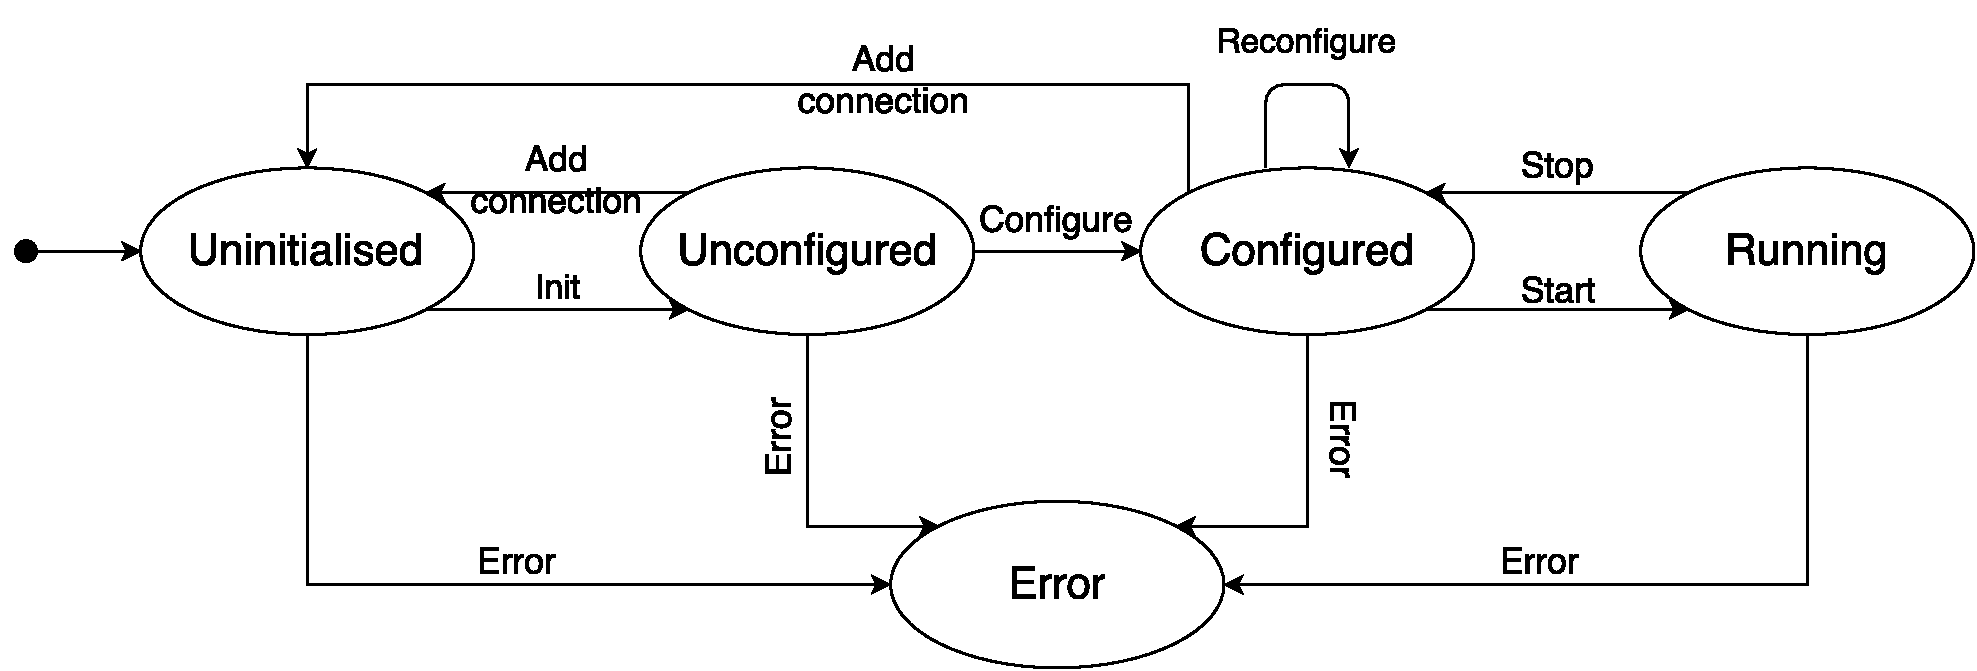
\includegraphics[width=0.9\textwidth]{src/images/fsmv2.pdf}
\end{center}
\caption{The FSM of EUDAQ.}
\label{fig:fsm}
\end{figure}

The \gls{FSM} is implemented in both the RunControl and the CommandReceiver (see \autoref{fig:fsm}) \cite{Shirokova:2016}. \\

Each CommandReceiver can always be characterized by the current state (\autoref{tab:statetab}).
\begin{table}
\centering
\small
\begin{tabular}{ l | l | l }
  \textbf{State} & \textbf{Enumerate Value} & \textbf{Acceptable Command} \\
  \hline
  \texttt{Error} & \texttt{eudaq::Status::STATE\_ERROR} & DoReset \\
  \texttt{Uninitialised} & \texttt{eudaq::Status::STATE\_UNINIT} & DoInitialise DoReset \\
  \texttt{Unconfigured} & \texttt{eudaq::Status::STATE\_UNCONF} & DoConfigure DoReset \\
  \texttt{Configured} & \texttt{eudaq::Status::STATE\_CONF} & DoConfigure DoStartRun DoReset \\
  \texttt{Running} & \texttt{eudaq::Status::STATE\_RUNNING} & DoStopRun \\
\end{tabular}
\caption{States of RunControl client.}
\label{tab:statetab}
\end{table}


The state of RunControl is determined by the lowest state of the connected client in the following priority: ERROR, UNINITIALISED, UNCONFIGURED, CONFIGURED, RUNNING. It means, for example, that even if only one connection is in the ERROR state, the whole machine will also be in that state. This prevents such mistakes as running the system before every component has finished the configuration.

\subsubsection{Command}\label{sec:command}

\begin{table}
\centering
\small
\begin{tabular}{ l | l | l | l |l }
  \textbf{Command} & \textbf{RunControl Side} & \textbf{Client Side} & \textbf{Pre State} & \textbf{State of Success}\\
  \hline
  \texttt{Initialise} & Initialise & DoInitialise & Uninitialised & Unconfigured\\
  \texttt{Configure} & Configure & DoConfigure & Unconfigured Configured & Configured\\
  \texttt{StartRun} & StartRun & DoStartRun & Configured & Running\\
  \texttt{StopRun} & StopRun & DoStopRun & Running & Configured\\
  \texttt{Reset} & Reset & DoReset & Error & Uninitialised\\
  \texttt{Terminate} & Terminate & DoTerminate & Any apart from Running & - \\
\end{tabular}
\caption{List of Commands.}
\label{tab:cmdtab}
\end{table}


\paragraph{Initialise}
When an EUDAQ process is in the state of Uninitialised, it accepts the Initialise command and executes the DoInitialise function provided by the user. When it is initialized, it does not accept further Uninitialised commands until it is reset to the Uninitialised state.

\paragraph{Configure}
When an EUDAQ process is in the state of Unconfigured or Configured, it accepts the Configure command and executes the DoConfigure function provided by the user. Please be aware that the second Configure command after a successful execution of the Configure command is allowed. It means the EUDAQ process is re-configurable but not re-initialisible.

\paragraph{StartRun}
When an EUDAQ process is in the state of Configured, it also accepts the StartRun command and executes the DoStartRun function provided by the user. In the case of the Producer, the Producer should talk to the hardware and produce and send Event data. In the case of the DataCollector, the DataCollector will get the Event stream from its connected Producer.

\paragraph{StopRun}
When an EUDAQ process is in the state of Running, it only accepts the StopRun command and executes the DoStopRun function provided by the user. RunControl will not send the StopRun command to the DataCollector until all Producers have returned from the DoStopRun function and feedback their status.

\paragraph{Reset}
In any case when an EUDAQ process goes to the state of Error, only the Reset command is allowed.

\paragraph{Terminate}
Except for the state of Running, the terminate command is allowed on all other states. When the Terminate command is called, the EUDAQ processes will be closed. If the user has to do something before exiting the EUDAQ process, this should be entered into the DoTerminate function which will then carry out the process before exiting.


% !TEX root = EUDAQUserManual.tex
\section{Writing a Producer}\label{sec:ProducerWriting}
Producers are the binding part between a user DAQ and the central EUDAQ Run Control. The base class of Producer is eudaq::Producer. The eudaq::Producer is an inherited class of eudaq::CommandReceiver which receives commands from the eudaq::RunControl. It also maintains a set of eudaq::DataSender comamnds which allow binary data (eudaq::Event) to be sent to each destination.\\

\subsection{Producer Prototype}\label{sec:Producer_hh}

\autoref{producerdef}, below, is part of the header file which declares the eudaq::Producer. You are required to write the user Producer derived from eudaq::Producer. According the the set of commands (\autoref{sec:command}) in the EUDAQ framework, there are six virtual functions which should be implemented in the user producer. They are DoInitialise(), DoConfigure(), DoStopRun(), DoStartRun(), DoReset() and DoTerminate(). These command-related functions should return as soon as possible since no further command can be execuseted until the current command is finished. \\

\lstinputlisting[label=producerdef, style=cpp, linerange=BEGINDECLEAR-ENDDECLEAR]{../../main/lib/core/include/eudaq/Producer.hh}

The virtual function Exec() can optionally be implemented in the user Producer. If this is not implemented, the default Exec() will connect to the RunControl and goes into an infinite loop and will only return when the Terminate command is executed. In case you are going to implement an Exec() function, please read the source code to find detailed information.

\subsection{Example Source Code: Dummy Event Producer}\label{sec:Ex0Producer_cc}
\subsubsection{Declaration}
Here we outline an example implementation of a user Producer. The full source code is available at file path user/example/module/src/Ex0Producer.cc.  \autoref{ls:ex0producerdef}, below, is the declaration part. There are six command related functions, a constructor function and a \texttt{Mainloop} function. \\

\lstinputlisting[label=ls:ex0producerdef, style=cpp, linerange=BEG*DEC-END*DEC]{../../user/example/module/src/Ex0Producer.cc}

The line \lstinline[style=cpp]{static const uint32_t m_id_factory = eudaq::cstr2hash("Ex0Producer")}, defines a static number which is a hash from the name string. This number will be used later as a ID to register this \lstinline[style=cpp]{Ex0Producer} to the EUDAQ runtime environment.

\subsubsection{Register to Factory}
To make the EUDAQ framework know of the existence of \lstinline[style=cpp]{Ex0Producer}, this Producer should be registered to \lstinline[style=cpp]{eudaq::Factory<eudaq::Producer>} with its static ID number. The input parameter types of the constructor function are also provided to the Register function. See the example code:
\lstinputlisting[label=ls:ex0producerdef, style=cpp, linerange=BEG*REG-END*REG]{../../user/example/module/src/Ex0Producer.cc}

\subsubsection{Constructor}
The Constructor function takes in two parameters, the runtime name of the instance of the Producer and the address of the RunControl. 
\lstinputlisting[style=cpp, linerange=BEG*CON-BEG*INI]{../../user/example/module/src/Ex0Producer.cc}
In this example of Ex0Producer, the constructor function does nothing beside passing parameters to the base constructor function of Producer and initializes the \lstinline[style=cpp]{m_exit_of_run} variable.

\subsubsection{DoInitialise}
This method is called whenever an initialize command is received from the RunControl. When this function is called, the correlated section of the initialization file have arrived to the Producer from the RunControl. This initialization section can be obtained by: \\
\lstinline[style=cpp]{eudaq::ConfigurationSPC eudaq::CommandReceiver::GetInitConfiguration()} \\

Here is an example \lstinline[style=cpp]{DoInitialise} of the Ex0Producer:
\lstinputlisting[style=cpp, linerange=BEG*INI-BEG*CONF]{../../user/example/module/src/Ex0Producer.cc}
The Configuration object \lstinline[style=cpp]{ini} is obtained. According to the value DUMMY\_STRING and DUMMY\_FILE\_PATH in \lstinline[style=cpp]{ini} object, a new file is opened and filled by dummy data. The path of the file is saved as a variable member for later access of this dummy data file.

\subsubsection{DoConfigure}
This method is called whenever a configure command is received from the RunControl. When this function is called, the correlated section of configuration file has arrived to the Producer from the RunControl. The configuration section named by the Producer runtime name can be obtained by:\\
\lstinline[style=cpp]{eudaq::ConfigurationSPC eudaq::CommandReceiver::GetConfiguration()} \\

Here is an example \lstinline[style=cpp]{DoConfigure} of Ex0Producer:
\lstinputlisting[style=cpp, linerange=BEG*CONF-BEG*RUN]{../../user/example/module/src/Ex0Producer.cc}
The variables \lstinline[style=cpp]{m_ms_busy}, \lstinline[style=cpp]{m_flag_ts} and \lstinline[style=cpp]{m_flag_tg} are set according to the Configuration object.

\subsubsection{DoStartRun}\label{sec:ex0prdstart}
This method is called whenever a StartRun command is received from the RunControl. When this function is called, the run-number has already been increased by 1. For a real hardware specific Producer, the hardware is told to startup.
Here is an example \lstinline[style=cpp]{DoStartRun} of Ex0Producer:
\lstinputlisting[style=cpp, linerange=BEG*RUN-BEG*STOP]{../../user/example/module/src/Ex0Producer.cc}
Instead of talking to real hardware, a file is opened. Then, a new thread is started using the function \lstinline[style=cpp]{Mainloop}.

\subsubsection{DoStopRun}
This method is called whenever a StopRun command is received from the RunControl. Here is an example \lstinline[style=cpp]{DoStopRun} of Ex0Producer:
\lstinputlisting[style=cpp, linerange=BEG*STOP-BEG*RST]{../../user/example/module/src/Ex0Producer.cc}

\subsubsection{DoReset}
When the Producer goes into an error state, only the Reset command is acceptable. It is recommended to reset all member variables to their original value when the producer object is instanced.\\
Here is an example \lstinline[style=cpp]{DoReset} of Ex0Producer: 
\lstinputlisting[style=cpp, linerange=BEG*RST-BEG*TER]{../../user/example/module/src/Ex0Producer.cc}
For any case the data thread is running, it should be stopped.

\subsubsection{DoTerminate}
This method is called whenever a StopRun command is received from the RunControl. After the return of \lstinline[style=cpp]{DoTerminate}, the application will exit.\\
Here is an example \lstinline[style=cpp]{DoStopRun} of Ex0Producer:
\lstinputlisting[style=cpp, linerange=BEG*TER-BEG*LOOP]{../../user/example/module/src/Ex0Producer.cc}
The data thread is then closed. 

\subsubsection{Send Event}
In \lstinline[style=cpp]{DoStartRun}, a data thread is created with the function \lstinline[style=cpp]{Mainloop}. Here is the implementation of this function. The generated data Event depends on the value set by \lstinline[style=cpp]{DoInitialise} and \lstinline[style=cpp]{DoConfigure}.
\lstinputlisting[style=cpp, linerange=BEG*LOOP-END*IMP]{../../user/example/module/src/Ex0Producer.cc}
In each loop, a new object of Event named Ex0Event is created. Trigger number and Timestamp are options to be set depending on the flags. A data block with 100 zeros is filled to the Event object by id 0. Another data block read from file is filled to some Event object by id 2. Then, this Event object is sent out by \lstinline[style=cpp]{SendEvent(std::move(ev))}. The first Event object has a flag BORE by the method \lstinline[style=cpp]{eudaq::Event::SetBORE()}

\paragraph{Tags}\label{sec:Tags}
The \texttt{Event} class also provide the option to store tags.
Tags are name-value pairs containing additional information which does not qualify as regular DAQ data which is written in the binary blocks.
Particularly in the \gls{BORE} this is very useful to store information about the exact sensor configuration which might be required in order to be able to decode the raw data stored.
A tag is stored as follows:
\begin{listing}
event.SetTag("Temperature", 42);
\end{listing}

The value corresponding to the tag can be set as an arbitrary type (in this case an integer),
it will be converted to a STL string internally.

\subsubsection{Error}\label{sec:Tags}
In the case when the Producer fails to run a command function an exception like this will be produced \\
\lstinline[style=cpp]{EUDAQ_THROW("dummy data file (" + m_dummy_data_path +") can not open for writing")}\\
An error message is then sent to the RunControl.



% !TEX root = EUDAQUserManual.tex
\section{Writing a DataCollector}\label{sec:DataCollectorWriting}
A DataCollector can take data from Producers and merge/synchronise those data.
A DataCollector consists of a CommandReceiver and a DataReceiver, where the first receives commands from the Run Control while the latter receives binary data events from one or more Producers. A dedicated synchronisation method should be implemented inside of the DataCollector to pack the incoming data.
The DataCollector base class is provided in order to simplify the integration. Example code for Producers is provided.

\subsection{DataCollector Prototype}\label{sec:datacollector_hh}

\autoref{ls:datacoldef}, below, is part of the header file which declares the eudaq::Producer. You are required to write the user DataCollector derived from eudaq::DataCollector.
There are nine virtual methods, belonging to two categories, which should be implemented by the user. The first category includes the methods \lstinline[style=cpp]{DoInitialise},
\lstinline[style=cpp]{DoConfigure}, \lstinline[style=cpp]{DoStopRun}, \lstinline[style=cpp]{DoStartRun}, \lstinline[style=cpp]{DoReset} and \lstinline[style=cpp]{DoTerminate} which are called by command received and should return as soon as possible. The other category includes the methods \lstinline[style=cpp]{DoConnect}, \lstinline[style=cpp]{DoDisconnect}, and \lstinline[style=cpp]{DoReveive} which respond to a connection in establishing or deleting, or a new coming Event.

\lstinputlisting[label=ls:datacoldef, style=cpp, linerange=BEG*DEC-END*DEC]{../../main/lib/core/include/eudaq/DataCollector.hh}

The virtual function Exec() is optional to be implemented in user DataCollector. Internally, the base Exec() to create two threads for command execution and data receiving,  itself then goes to an infinite loop and can never return until the Terminate command is executed. In case you are going to implement it yourselves, please read the source code to find detailed information.

\subsection{Example Code: DirectSave}\label{sec:directsavedatacollector_cc}
Here is an example code of a derived DataCollector, named DirectSaveDataCollector. As its name hints,  it does nothing except save all incoming Event data to disk directly. Printing out of the Event to screen is optional for debugging.
\lstinputlisting[label=ls:datacoldirsave, style=cpp]{../../main/module/std/src/DirectSaveDataCollector.cc}

Two virtual methods are implemented in DirectSaveDataCollector, \lstinline[style=cpp]{DoConfigure()} and \lstinline[style=cpp]{DoReceive(eudaq::ConnectionSPC id, eudaq::EventUP ev)}. It registers itself to the correlated \lstinline[style=cpp]{eudaq::factory} by the hash number from the name string \lstinline[style=cpp]{DirectSaveDataCollector}. 

\subsection{Example Code: SyncTrigger}\label{sec:ex2datacollector_cc}
Now, a more realistic example. The full source code is available here, \autoref{ls:ex2datacoldec}. It can merge the eudaq::Event by trigger number from the connected eudaq::Producer.
\lstinputlisting[label=ls:ex2datacoldec, style=cpp]{../../user/example/module/src/Ex0TgDataCollector.cc}
Compared to previous DirectSaveDataCollector example, two more virtual methods are implemented. They are \lstinline[style=cpp]{DoConnect}, \lstinline[style=cpp]{DoDisconnect}. The first, \lstinline[style=cpp]{DoConnect}, will be called when a new connection from eudaq::Producer is created, and the other, \lstinline[style=cpp]{DoDisconnect}, will be called  when the connection is expired. The information of the correlated connection is provided by the incoming parameter. The lifetime of the connection between the eudaq::DataCollector and eudaq::Producer is a data-taking run. No \lstinline[style=cpp]{DoConfigure} method is implemented, and this DataCollector is not Configurable.










% !TEX root = EUDAQUserManual.tex
\section{Writing a Data Converter}\label{sec:DataConverter}
As a framework, EUDAQ itself is developed with no knowledge of how hardware data can be decoded. Only the user can know the specific details of the readout data from hardware, so users are required to write a data converter derived from eudaq::DataConverter to convert to another format. The converted data can then be stored on disk or used as input data for any non-EUDAQ software.\\

Currently, as historical legacy, two different formats are provided along with the native raw eudaq::Event. They are eudaq::StandardEvent for pixel detectors, and eudaq::LCEvent as an EUDAQ wrapper for the LCIO format.

\subsection{Event Structure}
eudaq::Event is the most important data container in the EUDAQ system. eudaq::Event should be filled by detector data properly in order to transmit among eudaq clients, e.g.\ Producer and DataCollector. \autoref{tab:eventdata} lists all the member variables inside of eudaq::event. Not all of these variables have to be filled. For example, in case there is a trigger number but no timestamp information, the m\_ts\_begin and m\_ts\_end can be left untouched.

%%\begin{table}[!h]
%%{\footnotesize
%%\begin{tabular}{l|l|p{2cm}|p{5.5cm}}
%%Variable & Type & Default Value & Comment \\
%% \hline
%% m\_type & uint32\_t & - & Event type\\
%% m\_version & uint32\_t & - & Version of EUDAQ\\
%% m\_flag & uint32\_t & - & Event flag\\
%% m\_stm\_n & uint32\_t & - & Stream/device number\\
%% m\_run\_n & uint32\_t & - & Run number\\
%% m\_ev\_n & uint32\_t & - & Event number\\
%% m\_tg\_n & uint32\_t & - & Trigger number\\
%% m\_extend & uint32\_t & - & Reserved word\\
%% m\_ts\_begin & uint64\_t & - & Timestamp at the begin of trigger\\
%% m\_ts\_end & uint64\_t & - & Timestamp at the end of trigger\\
%% m\_dspt & std::string & - & Description String\\
%% m\_tags & std::map$<$std::string, std::string$>$& - & Tag pairs\\
%% m\_blocks & std::map$<$uint32\_t, std::vector$<$uint8\_t$>>$ & - & Raw data blocks\\
%% m\_sub\_events & std::vector$<$EventSPC$>$& - & Sub events\\
%% \end{tabular}
%% \caption{All member variables in eudaq::Event.}
%% \label{tab:eventvarialbe}
%% }
%% \end{table}
%% 
The eudaq::Event maye also have sub events. 

\subsubsection{RawDataEvent}\label{sec:convrawdata}
eudaq::RawDataEvent is derived from eudaq::Event with the m\_type always set to eudaq::cstr2hash(``RawDataEvent''). It has the same member variables and functions as the base eudaq::Event. However the member variable m\_extend is used as an identification number of the sub type of event.

\subsubsection{StandardEvent}\label{sec:convstddata}
eudaq::StandardEvent is derived from eudaq::Event with the m\_type always set to eudaq::cstr2hash(``StandardEvent''). Historically, it presents a beam telescope tracking-hit event with all hit information of sensor planes. The hit information is contained by eudaq::StandardPlane. The beam telescope planes are pixel sensors. The spatial position and signal amplitude of the fired pixels are zero-compressed inside eudaq::StandaredPlane.

\subsection{Example Code: RawEvent2StdEvent}\label{sec:Ex0RawEvent2StdEventConverter_cc}
This example DataConverter is named Ex0RawEvent2StdEventConverter. As indicated by the name, it converts the eudaq::RawDataEvent to eudaq::StandardEvent. The sub type of eudaq::RawDataEvent is ``my\_ex0'' which is also used to calculate the hash and register it to the eudaq::Factory. If an eudaq::RawDataEvent object announcing its sub-type by ``my\_ex0'' exists when doing the data converting, this object will be forwarded to that Ex0RawEvent2StdEventConverter.
\lstinputlisting[label=ls:ex0raw2std, style=cpp]{../../user/example/module/src/Ex0RawEvent2StdEventConverter.cc}


\subsection{RawEventTTreeEvent Converter}\label{sec:Ex0RawEvent2TTreeEventConverter_cc}

Another working example of converting the {\tt raw} event to {\tt ROOT TTree} format is also provided. The details and flow of converter is described in Annexe 1. 

% !TEX root = EUDAQUserManual.tex
\section{Writing a Monitor}\label{sec:MonitorWriting}
eudaq::Monitor provides the the base class and common methods to monitor the data quality online. The internal implementation of eudaq::Monitor is very similar to eudaq::DataCollector. The only difference between them is that eudaq::Monitor accepts only a single connection from an eudaq::DataCollector or eudaq::Producer. (not implemented)\\

\subsection{Monitor Prototype}\label{sec:monitor_hh}

\lstinputlisting[label=ls:monitordef, style=cpp, linerange=BEG*DEC-END*DEC]{../../main/lib/core/include/eudaq/Monitor.hh}

\subsection{Example Code}
Here is an example code of a derived Monitor, named Ex0Monitor. It gets configration paratmeter at configration time and do print out the infomation of the received Events. It might do an Event converting depending on how it is configured.
\lstinputlisting[label=ls:ex0monitorcc, style=cpp]{../../user/example/module/src/Ex0Monitor.cc}
Two virtual methods are implemented in Ex0Monitor, \lstinline[style=cpp]{DoConfigure()} and \lstinline[style=cpp]{DoReceive(eudaq::EventUP ev)}. It registers itself to the correlated \lstinline[style=cpp]{eudaq::factory} by the hash number from the name string \lstinline[style=cpp]{Ex0Monitor}.

\subsection{Graphical User Interface}
Normally, to monitoring the data quality, graphic plots are required. It means that an external graphic library is required. ROOT, Qt
and gnuplot can be the possible graphic library.

\subsubsection{StdEventMonitor}
StdEventMonitor is an EUDAQ version 1 legacy. It was named as OnlineMonitor. Actually, it can only display the plots from StandardEvent. If the Converter to StandardEvent of the incoming Event exists, StdEventMonitor will call the correlated Converter and do the converting itself.
StdEventMonitor depends ROOT to generate and plot graph.

% !TEX root = EUDAQUserManual.tex
\section{Writing a RunControl}\label{sec:RunControlWriting}
In most user cases, the base eudaq::RunControl can meet the requirements of the controlling flow process to the detector system which use the EUDAQ framework. It is still possible to override the default behavior of the base eudaq::RunControl by implementing a derived RunControl class.

\subsection{RunControl Prototype}
The command methods are \lstinline[style=cpp]{Initialise()}, \lstinline[style=cpp]{Configure()}, \lstinline[style=cpp]{StartRun()}, \lstinline[style=cpp]{StopRun()}, \lstinline[style=cpp]{Reset()} and \lstinline[style=cpp]{Terminate()}. \\

The methods \lstinline[style=cpp]{DoConnect()}, \lstinline[style=cpp]{DoDisconnect()}, \lstinline[style=cpp]{DoStatus()} are also provided for the case where the derived RunControl wants to be informed of any connection change and the object eudaq::Status is sent to the RunControl.\\

\subsection{Example Code: auto stop}
Here is an example code of a derived RunControl, named Ex0RunControl. It can check the elapsed time after the start of data taking, and stop the data taking after a configurable time period.
\lstinputlisting[label=ls:ex0runcontrolcc, style=cpp]{../../user/example/module/src/Ex0RunControl.cc}
4 virtual methods are override in Ex0Monitor: \lstinline[style=cpp]{Configure()}, \lstinline[style=cpp]{StartRun()}, \lstinline[style=cpp]{StopRun()} and \lstinline[style=cpp]{Exec()}. It registers itself to the correlated \lstinline[style=cpp]{eudaq::factory} by the hash number from the name string \texttt{Ex0RunControl}.

\subsection{RunControl Mode}
There are two options when making the integration of the EUDAQ RunControl and other DAQ systems which do not adapt the eudaq::Producer approach and can not talk with base eudaq::RunControl. The Ex0RunControl example is working the first case.
\subsubsection{EUDAQ Working as Master DAQ}
In this case, the RunControl should behave as an entrance point to the full detector system. As the base eudaq::RunControl can not manage the controlling of the non-EUDAQ slave DAQ, users are required to implement a specific RunControl class derived from eudaq::RunControl. With overloaded virtual methods, the user RunControl not only governs the EUDAQ system but also talks to the non-EUDAQ component by user specific communication protocols.\\
By this approach, the user RunControl can be instanced by the standard GUI RunControl launcher (euRun).

\subsubsection{EUDAQ Working as Slaver DAQ}
In this case, the base eudaq::RunControl can be left as is without modification or derivation. However, the standard GUI RunControl launcher is not usable. The master DAQ should instance an object
of eudaq::RunControl and call the correlated method whenever it wants to issue the command to the EUDAQ subsystem and get the status report.




% !TEX root = EUDAQUserManual.tex
\section{Support User Defined Event Type}\label{sec:NewDataHandling}
In the EUDAQ framework, the definition \texttt{data} usually means an object of eudaq::Event or its derivations. 

\subsection{Event}
eudaq::Event is serializable as it is derived from eudaq::Serializable and implements
\begin{listing}
  Event(Deserializer &);
  virtual void Serialize(Serializer &) const;    
\end{listing}

There are three eudaq::Event derivations in the default installation of EUDAQ. They are \lstinline[style=cpp]{RawDataEvent} (\autoref{sec:convrawdata}), \lstinline[style=cpp]{StandardEvent} (\autoref{sec:convstddata}) and \lstinline[style=cpp]{LCEvent}. The eudaq::Event derivations are serializable. But if there are additional member variables introduced to derived Events, the new variable should be serialized along with the other variables defined in eudaq::Event. If this is not done, the unserialized data will be lost.

It is recommend to reuse the raw data blocks \lstinline[style=cpp]{m_blocks} of eudaq::Event. Then the base eudaq::Event will serialize and deserialize the \lstinline[style=cpp]{m_blocks}.\\

\subsection{FileWriter}\label{sec:FileWriterWriting}
Usually, the objects of eudaq::Event and its derivations are the only data going to be stored in disk for later offline analysis. The user may prefer to write Event data in other format which is human readable or widely used by other software. In order to define a new file format, the user can define a class derived from eudaq::FileWriter.


\subsubsection{FileWriter Prototype}
\lstinputlisting[label=ls:filewritedec, style=cpp, linerange=BEG*DEC-END*DEC]{../../main/lib/core/include/eudaq/FileWriter.hh}

\subsubsection{Example Code: NativeFileWriter}
No matter if the user defined Event reuses the \lstinline[style=cpp]{m_blocks} raw data block or does serialization of new variables itself, it can write to disk in binary format (aka native) which can only be read by EUDAQ.

\lstinputlisting[label=ls:rawfilewritecc, style=cpp]{../../main/lib/core/src/NativeFileWriter.cc}

\subsection{FileReader}\label{sec:FileReaderWriting}
To reconstruct the Event from a disk file in native format or user-defined format, the class eudaq::FileReader is provided. Each writing data format should have its correlated implementation of FileReader to access the disk file.

\subsubsection{FileReader Prototype}
\lstinputlisting[label=ls:filereaderdec, style=cpp, linerange=BEG*DEC-END*DEC]{../../main/lib/core/include/eudaq/FileReader.hh}

\subsubsection{Example Code: NativeFileReader}
\lstinputlisting[label=ls:rawfilereadercc, style=cpp]{../../main/lib/core/src/NativeFileReader.cc}

%% % !TEX root = EUDAQUserManual.tex
\section{Usefull Utilities}
The EUDAQ framework contains a number of other parts that may be useful.
Those that have not already been described in previous sections will be outlined below.\\


There are a number of other utilities available that are not needed for running the DAQ,
but can be useful for other tasks such as debugging.
The executables are all located in the \texttt{bin} subdirectory.
They should all accept a help (\texttt{-h} or \texttt{--help}) option,
to print a summary of the available options.


\subsection{FileChecker}
\label{sec:FileChecker}

This is a small utility that reads raw data files and checks if all events are
readable, can be syncronised using the TLU trigger id and lists which type
of subevents the file contains.

It should be called with list of file paths or run numbers. For any argument
that consist only of numerical digits the file path is constructed by
substituting \texttt{\$6R} in the input pattern (defaults to
``\texttt{../data/run\$6R.raw}'') with the run number padded to 6 digits.

For example:
\begin{listing}[mybash]
$[./FileChecker]$ {6045..6050}
\end{listing}

This would produce the following output.
\begin{listing}[]
run     valid  num_events  contains                   errors                    
------  -----  ----------  -------------------------  ----------------------
  6045   true       13131  MUPIX4,NI,TLU                                        
  6046   true           1  MUPIX4,NI,TLU                                        
  6047   true       14674  MUPIX4,NI,TLU                                        
  6048   true        7776  MUPIX4,NI,TLU                                        
  6049  false           0                             no events in the file.    
  6050  false          -1                             read error. 
\end{listing}


\subsection{Converter}
\label{sec:Converter}
The \texttt{Converter} program will read a native data file,
optionally select just a subset of events from the file,
and can then write it out to another file in either the same native format, or a different format.
The most commonly used options are:
\begin{description}
\ttitem{-t \param{type}}
The file type to write out.
The available types are listed below.

\ttitem{-e \param{range}}
Select the specified range of event numbers.

\ttitem{-s}
Try to resynchronize events based on the TLU event number
(see TestReader in \autoref{sec:TestReader}).

\end{description}

The available output file types are as follows:

\begin{description}\phantomsection\label{lst:FileTypes}

\ttitem{native}
The native EUDAQ binary file format, consisting of a serialised stream of
\texttt{DetectorEvent}s, containing the raw data read out from the hardware.

\ttitem{standard}
Like the \texttt{native} format, this is also a serialised stream,
but in this case it contains \texttt{StandardEvent}s,
in which the raw data has been converted into a standard format.

\ttitem{lcio}
The standard \gls{LCIO} file format used by the analysis software.
This type is only available if EUDAQ was compiled with \gls{LCIO} support.

\ttitem{root}
A Root file containing a TTree with the hit pixel information.

\ttitem{text}
A simple text based format (not yet implemented).

\ttitem{mimoloop}
A text based format mimicking the output of the mimoloop program
(from Angelo Cotta Ramusino and Lorenzo Chiarelli at INFN Ferrara).

\end{description}

Although this program can be used to convert a native data file into \gls{LCIO} format,
the more usual (and therefore better tested) way is to use the EUTelescope converter.

\subsection{ClusterExtractor}
\label{sec:ClusterExtractor}
This program can be used to quickly extract some clusters from raw data.
It is not as sophisticated as the EUTelescope package, which should be preferred for real analysis,
but it can be useful for doing quick checks.
It will read a native data file, perform a basic clustering,
and then write these clusters to one text file per sensor plane.
The most commonly used options are:
\begin{description}
\ttitem{-p \param{pixels}}
The cluster size in pixels.
It should be an odd number, with 1 meaning no clustering (just pixels over threshold),
3 meaning 3\x{}3 pixel clusters, etc.

\ttitem{-n \param{adcs}}
The noise level (sigma) in ADC units.
This is used to scale the thresholds in terms of the noise.

\ttitem{-s \param{thresh}}
The threshold for seed pixels, in terms of the noise.

\ttitem{-c \param{thresh}}
The threshold for the total charge of a cluster,
in terms of the cumulative noise of all the pixels in the cluster.

\ttitem{-w}
Reports the cluster centre as the weighted average of the pixels,
instead of the position of the seed pixel.

\end{description}

An example use is:
\begin{listing}[mybash]
$[./ClusterExtractor]$ -p 3 -n 3.5 -s 6 -c 10 -w 5432
\end{listing}

This will generate a number of text files named \texttt{runNNN\_eutel\_M.txt},
where \texttt{NNN} is the run number, and \texttt{M} is the sensor plane number.
The format of the output text files is as follows:
\begin{listing}[]
2       2       51487659237
 182    153     126
 241    120     125
3       1       51489095892
 111    67      346
5       1       51491334074
 113    141     171
7       2       51495330212
 252    240     305
 95     170     189
\end{listing}

The first line contains the event number,
the number of clusters, and the TLU timestamp.
Then for each cluster there is one line,
containing the \texttt{x} and \texttt{y} coordinates of the cluster centre,
and the total charge in ADC units.
The cluster lines are prepended with a space to make it easier to scan the file by eye.


\subsection{MagicLogBook}
\label{sec:MagicLogBook}
This program is designed to extract as much information as possible from data files and log files,
in order to reconstruct a log book.
Despite its name, it is in fact not magical,
so it is preferable to keep a good log book during running,
rather than relying on this program to generate it later.

The available options are listed below:
\begin{description}
\ttitem{-f \param{fields}}
A list of fields to include in the output, in the form \texttt{name=value},
with multiple fields separated by commas.
If a predefined list is also specified these will be appended to the list.

\ttitem{-s \param{separator}}
The separator to use between fields in the output. The default is a tab character.

\ttitem{-h \param{string}}
A string that appears at the beginning of the header line (with the list of field names),
that can be used to differentiate it from the other lines. The default is an empty string.

\ttitem{-p {name}}
Use a predefined list of fields.
Currently available values are \texttt{normal} and \texttt{full}.

\ttitem{-o \param{file}}
The output filename. By default the standard output is used.

\end{description}

The easiest method of running is to use a predefined list of fields.
There are currently two predefined lists available: \texttt{normal} and \texttt{full}.
If neither of these are suitable, contact the EUDAQ maintainer,
as it may be possible to add more options.

The \texttt{normal} list includes:
\begin{myitemize}
  \item the run number,
  \item the config file name,
  \item the run start time,
  \item for the \glspl{EUDRB}:
  \begin{myitemize}
    \item the mode,
    \item the sensor type,
    \item whether they are running unsynchronized,
    \item the number of boards,
    \item and the firmware version.
  \end{myitemize}
  \item and for the \gls{TLU}:
    \begin{myitemize}
    \item the internal trigger interval,
    \item the AND mask,
    \item the DUT mask,
    \item and the firmware version.
  \end{myitemize}
\end{myitemize}

The \texttt{full} list includes all the values from the \texttt{normal} list,
plus the number of events in the run and the end of run time.
This is because these values can only be known by reading
the whole data file to the end, which is slow, especially for large data files.

If necessary, other information is available using custom fields,
although the syntax for these is a bit complicated,
since it is designed to be as flexible as possible at specifying any information in the data file.
In the future it may be redefined in order to simplify it if possible.
Therefore it is recommended to use a predefined list of fields where possible.
Custom fields are specified as a comma separated list of items in the form \texttt{name=value},
with the name being what will appear on the header line of the output,
and the value specifying what exactly to extract from the file.
The possible values are illustrated below, although not exhaustively:

\begin{mydescription}
  \ttitem{events$^\ast$} The number of events in the run.
  \ttitem{config} The configuration name, or:
  \begin{mydescription}
    \ttitem{config:section:key} The value of the \texttt{key} from the corresponding \texttt{section} in the config
    (e.g. \texttt{config:Producer.EUDRB:NumBoards}).
  \end{mydescription}
  \item{\texttt{bore}, \texttt{tlu}, \texttt{eudrb}, \texttt{eore}$^\ast$:} Something from the \gls{BORE},
  the \texttt{TLUEvent} or \texttt{EUDRBEvent} subevents of the \gls{BORE}, or the \gls{EORE}, respectively:
  \begin{mydescription}
    \ttitem{bore:.Run} The run number
    \ttitem{bore:\param{name}} Otherwise, if the second part does not start with a period, the value of the tag \param{name} is used
    (e.g. \texttt{tlu:DutMask} or \texttt{eudrb:MODE}).
  \end{mydescription}
  \ttitem{log} Something from the log file (not implemented yet).
\end{mydescription}

$^\ast$ items marked with an asterisk require reading the whole data file, and are therefore slow,
especially when large data files are involved.

Note that the \texttt{EUDRBEvent} is now deprecated, having been replaced by the \texttt{RawDataEvent},
but there is currently no way to specify this.

The \texttt{MagicLogBook} command is used as follows:

\begin{listing}[mybash]
$[./MagicLogBook]$ -p normal ../data/*.raw
\end{listing}

This will produce an output similar to the following:
\begin{listing}[]
Run  Config     Mode Det Start                   U P Trg AND  DUT  Tfw Efw
6371 eudet-beam          2009-07-29 07:44:39.535 1 6   0 0xf  0x10 241
6372 eudet-beam          2009-07-29 08:03:05.079 1 6   0 0xf  0x10 241
6373 eudet-m26test       2009-07-30 09:57:45.157 1 6 255 0xff 0x12 241
6374 eudet-m26test       2009-07-30 10:00:45.205 1 6 255 0xff 0x12 241
6375 eudet-m26test       2009-07-30 10:05:38.625 1 6   1 0xff 0x12 241
6376 eudet-m26test       2009-07-30 10:10:00.107 1 6   1 0xff 0x12 241
6379 eudet-m26test       2009-07-30 10:13:05.322 1 6   1 0xff 0x12 241
\end{listing}

Note that the header row has been modified slightly to fit into the page width:
the \texttt{U} should be \texttt{UnSync}, \texttt{P} should be \texttt{Planes},
\texttt{Trg} should be \texttt{TriggerInterval}, \texttt{Tfw} should be \texttt{TLUfw},
and \texttt{Efw} should be \texttt{EUDRBfw}.
The columns \texttt{Mode}, \texttt{Det} and \texttt{EUDRBfw} are missing from the output
due to the fact that this information is now stored in a \texttt{RawDataEvent},
which is not currently accessible with this version of the program.


\subsection{PluginManager}\label{sec:PluginManager}
The \texttt{PluginManager} handles the different \texttt{DataConverterPlugin}s,
allowing raw data stored in a \texttt{RawDataEvent} to be easily converted
to a \texttt{StandardEvent} or \texttt{LCEvent} without having to know the details of all the detector types in there.
It is defined in the following header:
\begin{listing}
#include "eudaq/PluginManager.hh"
\end{listing}

In order to convert the events correctly,
the plugins must have access to the information in the BORE.
Therefore, before any events may be converted, and for each data file,
the \texttt{PluginManager} must be initialized as follows:
\begin{listing}
eudaq::PluginManager::Initialize(bore);
\end{listing}

The \texttt{PluginManager} will take care of passing the relevant parts of the \gls{BORE}
to the appropriate \texttt{DataConverterPlugin}s.
The \texttt{DetectorEvent}s can then be converted as follows:
\begin{listing}
eudaq::StandardEvent sev = eudaq::PluginManager::ConvertToStandard(dev);
\end{listing}

The \texttt{PluginManager} will take care of splitting the \texttt{DetectorEvent}
into its constituent subevents, and passing them all to the appropriate
\texttt{DataConverterPlugin}s to be inserted into the returned \texttt{StandardEvent}.
For a slightly more complete example of the \texttt{PluginManager},
see the \texttt{ExampleReader} in \autoref{sec:ExampleReader}.

\subsection{OptionParser}
The \texttt{OptionParser} is used to simplify parsing of command-line options.
It provides a way to specify which arguments a program accepts,
with the types, default values and descriptions,
so that the help text can be automatically generated,
and therefore is always in sync with the code,
and all command line programs can have a uniform interface.

All programs using the \texttt{OptionParser} will automatically provide a
\texttt{-h} (and \texttt{--help}) option to display the help text,
as well as a \texttt{-v} (and \texttt{--version}) option to display the program version,
unless the program explicitly overrides these options with other ones with the same names.

The \texttt{OptionParser} is the class that handles the actual parsing of the command line.
The signature of the constructor is as follows:
\begin{listing}
OptionParser(const std::string & name, const std::string & version,
             const std::string & desc="", int minargs = -1, int maxargs = -1);
\end{listing}
The first three arguments are the program name, version and (optionally) description,
and these are optionally followed by two numbers specifying the number of arguments
expected after the command line options.
The default value of -1 for the minimum means no arguments are allowed,
and for the maximum means that an arbitrary number may be given
(i.e. there is no explicit maximum).

If the automatically generated help text is not sufficient,
extra text may also be given to display at the end of the help text,
by passing it to the following method:
\begin{listing}
void OptionParser::ExtraHelpText(const std::string & text);
\end{listing}
This can be used to provide extra information about the options to the program.

Once an \texttt{OptionParser} object has been constructed, the different options may be specified.
There are two types: \texttt{OptionFlag}, which specifies a simple option with no argument,
and the template \texttt{Option<T>}, which specifies an option taking an argument of type \texttt{T}.

The \texttt{OptionFlag} constructor has the following signature:
\begin{listing}
OptionFlag(OptionParser & op, const std::string & shortname,
           const std::string & longname, const std::string & desc = "");
\end{listing}
where \texttt{op} is a reference to the \texttt{OptionParser} object created previously,
that will do the actual parsing of the command line.
It then takes two names: a short version (usually a single character) that is used with a single hyphen,
and a long version that must be preceded by two hyphens on the command line.
Finally, a description may be given that will be displayed in the help text.

The \texttt{Option} constructor has the following two signatures,
one for normal types, the other for vectors of another type:
\begin{listing}
Option<T>(OptionParser & op, const std::string & shortname,
          const std::string & longname, const T & deflt = T(),
          const std::string & argname = "", const std::string & desc = "");
Option<std::vector<T> >(OptionParser & op, const std::string & shortname,
          const std::string & longname, const std::string & argname = "",
          const std::string & sep = "", const std::string & desc = "");
\end{listing}
where, in both cases, the first three arguments are as for \texttt{OptionFlag}.
The first constructor then takes a default value that will be used
in the case the option is not specified on the command line,
a name for the argument to the option (to be used in the help text),
and a description of the option.
The vector version also takes an argument name and a description,
but no default value (the default is always an empty vector), instead it takes a separator,
which is the string used to separate multiple elements of the vector on the command line.
By default (or if an empty string is specified), a comma will be used.

Once all the options have been specified, the command line can be parsed,
which is done by calling the following method of the \texttt{OptionParser} object:
\begin{listing}
OptionParser & OptionParser::Parse(const char ** args);
\end{listing}
as an argument it takes the list of arguments from the command line (by convention usually called \texttt{argv}).
If there is an error during parsing, an exception may be thrown;
this should be handled by the \texttt{HandleMainException} method as described below.

Afterwards the values of the options can be accessed using their \texttt{Value()} method.
The \texttt{IsSet()} method is also available to tell whether an option has been set on the command line
(for \texttt{OptionFlag}s this will hold the same value as the \texttt{Value()} method).

Finally, the \texttt{OptionParser} has a \texttt{HandleMainException} method that provides
a way to catch any unhandled exceptions,
and either display help if it is a problem with parsing the command line,
or otherwise display a standard text informing the user of a problem.
It will also catch exceptions of type \texttt{MessageException} and display the message,
without treating it as an error, so this can be used to exit the program with a message to the user.
It is recommended to put the main program inside a \texttt{try} block,
then call the \texttt{HandleMainException} method from a \texttt{catch(...)} block,
after any other exceptions have been handled (if necessary).

An example use is shown below, illustrating most of what is described above:
\lstinputlisting[style=full, language=C++]{../../main/exe/src/OptionExample.cxx}

Running this program produces the following output:
\begin{listing}[mybash]
$[./OptionExample.exe]$ -h
Example version 1.0
An example program

usage: ./OptionExample.exe [options] [0 or more arguments]

options:
  -t --test
     Enable test
  -e --example <value>	(default = 42)
     Example parameter
  -a --another <values>	(default = )
     Example vector

Some more information about this program.

$[./OptionExample.exe]$
Test: Disabled
Example: 42
Another: 
No arguments were given

$[./OptionExample.exe]$ -t -e 2.718 -a 1;2;3 foo bar
Test: Enabled
Example: 2.718
Another: 1, 2, 3
Argument 1: foo
Argument 2: bar
\end{listing}

\subsection{Timer}
The \texttt{Timer} class wraps the underlying operating system's timer functions,
making them easier to use in a platform independent way.
Whenever a \texttt{Timer} object is created, it will record the current time.
Then at any time in the future, the elapsed time in seconds may be accesses
with the \texttt{Seconds()} method.

There is also a \texttt{Stop()} method to stop the timer counting, so any subsequent calls
to \texttt{Seconds} will return the same value, and a \texttt{Restart()} method to
reset the timer's start time to the current time and start counting again.
An example use is shown below:
\begin{listing}[C++]
#include "eudaq/Timer.hh"

Timer t;
function_a();
cout << "Function A took " << t.Seconds() << " seconds." << endl;
t.Restart();
function_b();
cout << "Function B took " << t.Seconds() << " seconds." << endl;
// wait 3 microseconds
t.Restart();
while (t.Seconds() < 3e-6) {
  // do nothing
}
\end{listing}

This shows a timer being used to measure the execution time of two functions,
and to wait for a small delay.
Usually to wait for a delay, it is preferable to use sleep (or \texttt{mSleep}, see \autoref{sec:mSleep}),
but in most operating systems the minimum delay for a sleep is around 20~ms
(even when using \texttt{usleep} which has microsecond resolution)
so if the delay must be shorter, a busy loop like above is needed.

\subsection{Utils}
The \texttt{Utils} package is a collection of useful functions and classes too small to merit
their own individual files.
It is used by including the header:
\begin{listing}
#include "eudaq/Utils.hh"
\end{listing}

Some of the most useful parts are described here.

\subsubsection{to\_string}
This is a template function that takes (almost) any type and returns the value converted to a string.
An optional second argument specifies the minimum number of digits to use
(padding with zeroes if necessary).
\begin{listing}
int value = 123;
strfunction(to_string(value));
strfunction(to_string(value, 6));
\end{listing}

This will pass first the string \inline{"123"},
and then the string \inline{"000123"}
to the function \texttt{strfunction}.

\subsubsection{from\_string}
This template function is the inverse of \texttt{to\_string}.
It takes as arguments a string and a default value of type T,
and returns an object of type T initialised from the string.
If it is not possible to convert the string to the required type,
the default value is returned instead.
\begin{listing}
std::string value = "456";
intfunction(from_string(value, 0));
\end{listing}

This will call \texttt{intfunction} with the integer value 456.

\subsubsection{hexdec}
This is a class to facilitate printing numbers in both hexadecimal and decimal.
It is used similarly to \texttt{to\_string}, but when printed,
it will display the value in hexadecimal, followed by the value in decimal in parentheses.
The hexadecimal values will be padded to the full width of the type,
unless a second argument is given specifying the minimum number of hex digits to display.
\begin{listing}
short value = 789;
cout << hexdec(value) << endl
     << hexdec(value, 0) << endl;
\end{listing}

This will display:
\begin{listing}[]
0x0315 (789)
0x315 (789)
\end{listing}

If the result is required in a string, instead of being printed,
this can be achieved with \inline{to_string(hexdec(value))}.

\subsubsection{mSleep}\label{sec:mSleep}
This is a wrapper around the operating system's \texttt{sleep}/\texttt{usleep}
(or equivalent) function.
It takes as an argument the number of milliseconds to sleep.
The advantage of this function is that it will work on Linux,
Mac OS X and Windows, as it will automatically call the correct underlying function.

\subsection{Python Interface}
\label{sssec:pywrapper}
A Python interface is provided for selected EUDAQ components:
RunControl, DataCollector and a Producer, that can be extended on the
Python side. The interface is realized through the \texttt{ctypes}
package that is part of every standard Python installation and
requires the \texttt{numpy} Python package to be installed. The
interface code for all components is located in the
\texttt{main/python} directory.

To use the interface and access the components as Python objects, the
wrapper must be loaded inside your Python script:

\begin{listing}[python]
  #!/usr/bin/env python2 
  execfile('PyEUDAQWrapper.py') # load ctypes wrapper

  prc = PyRunControl() # start run control with default settings
  # wait for more than one active connection to appear
  while prc.NumConnections < 2:
      sleep(1)
  prc.Configure("ExampleConfig") # load configuration file
  while not prc.AllOk:
      sleep(1) # sleep while waiting for all connected producers
  prc.StartRun()
\end{listing}

This little scripts creates a RunControl instance, sends a
configuration to all connected producers, waits for their reply, and
starts a new run. Several more extensive examples for using Python
with EUDAQ are located in the \texttt{python} directory in the main
EUDAQ directory.

\subsection{Log Messages}
The logging infrastructure allows to send information, error messages or debug information to a central point in the DAQ system to collect logging information, the Log Collector.
It is strongly encouraged to use the logging system rather than simple cout statements.
The logging class is defined in:
\begin{listing}
#include "eudaq/Logger.hh"
\end{listing}

The following macros for sending log messages are defined,
listed here in decreasing order of severity:
\begin{description}

\ttitem{EUDAQ\_USER}
A user-generated message (e.g. from the RunControl Log button).

\ttitem{EUDAQ\_ERROR}
Something that went wrong and should be fixed. Errors usually are blocking, i.e. the data acquisition cannot be continued without fixing the cause.

\ttitem{EUDAQ\_WARN}
A warning that something may not be quite right and should probably be taken care of. Warnings are considered non-blocking, i.e. the data acquisition will proceed but some of the components might experience problems (lacking configurations for a threshold setting would be an example).

\ttitem{EUDAQ\_INFO}
An message generated during normal running containing information that may be useful to the user.

\ttitem{EUDAQ\_EXTRA}
Some extra information that may be less useful in normal running.

\ttitem{EUDAQ\_DEBUG}
Information for debugging purposes that will normally be hidden and should only be used for development purposes. Additional information for shifters should be categorized as \texttt{EUDAQ\_EXTRA}.

\end{description}

They are used as follows:
\begin{listing}
EUDAQ_ERROR("No keyboard detected: press F1 to continue.");
\end{listing}

The messages will be sent to the central Log Collector if it is connected,
otherwise they will be displayed on the local terminal.
The log level can be changed in the following way:
\begin{listing}
EUDAQ_LOG_LEVEL("WARN");
\end{listing}

Any messages lower than the specified level will just be ignored.
This can be useful to filter out unimportant messages and, for example, just display error messages.

% !TEX root = EUDAQUserManual.tex
\section{Contributing to EUDAQ}
\label{sec:contributing}

\subsection{Reporting Issues}
\label{sec:reporting}
The GitHub server, on which EUDAQ is hosted, provides a system for reporting bugs and for requesting new features.
It is accessible at the following address: 

\url{https://github.com/eudaq/eudaq/issues}.

Here you may submit new reports (you are required to register first to do this),
or follow the status of existing bugs and feature requests.
This is recommended over (or at least, as well as) sending an email to the developers,
as it ensures a record of the issue is available, and others may follow the progress.

\subsection{Regression Testing}
\label{sec:ctest}

If a CMake version later than 3.1 is found and Python is installed
together with the \texttt{numpy} package, several regression tests are made
available that can be executed through CTest. The tests are based on
the Python wrapper around EUDAQ components as described in
section~\ref{sssec:pywrapper}. Run the tests by typing

\begin{listing}[mybash]
  cd build
  cmake ..
  ctest
\end{listing}

This starts the script \texttt{etc/tests/run\_dummydataproduction.py}
which runs a short DAQ session with instances of RunControl,
DataCollector and a (dummy) Producer and compares the output to a
reference file stored on AFS at DESY. If your system is set up
correctly, you have access to the reference file, and the basic
components of the EUDAQ library work, all tests should pass.
To see the output of failing tests, you can add the
\texttt{--output-on-failure} parameter to the CTest command.

These basic tests can easily be extended to test other parts of the
core framework or of your own producer. Take a look at the
\texttt{etc/tests/testing.cmake} CMake script and the central
\texttt{CMakeLists.txt} file where it is included for an example of
how to set up tests with CTest.

The automated nightly tests are defined in CMake scripts located in
\texttt{etc/tests/nightly} and are executed by the scripts
\texttt{run\_nightly.sh} and \texttt{run\_nightly.bat} for Unix and
Windows platforms, respectively. In addition to the dummy run
described above, the nightly tests check out all changes from the
central repository, build the full code base, and submit all results
to the CDash webserver hosted at DESY: \url{http://aidasoft.desy.de/CDash/index.php?project=EUDAQ}

\subsection{Commiting Code to the Main Repository}
\label{sec:commiting}



If you would like to contribute your code back into the main repository, please follow the ``fork \& pull request'' strategy:

\begin{itemize}
\item Create a user account on github, log in
\item ``Fork'' the (main) project on github (using the button on the page of the main repo)
\item \emph{Either}: clone from the newly forked project and add
  'upstream' repository to local clone (change user names in URLs
  accordingly):
  \begin{listing}[mybash]
git clone https://github.com/your_account_name/eudaq eudaq
cd eudaq
git remote add upstream https://github.com/eudaq/eudaq.git
\end{listing}
\item \emph{or} if edits were made to a previous checkout of upstream: rename origin to upstream, add fork as new origin:

  \begin{listing}[mybash]
cd eudaq
git remote rename origin upstream
git remote add origin https://github.com/your_account_name/eudaq
git remote -v show
\end{listing}
\item Optional: edit away on your local clone! But keep in sync with
  the development in the upstream repository by running
  \begin{listing}
git fetch upstream        # download named heads or tags
git pull upstream master  # merge changes into your branch
\end{listing}
on a regular basis. Replace \texttt{master} by the appropriate branch if you work on a separate one.
Don't forget that you can refer to issues in the main repository anytime by using the string \texttt{eudaq/eudaq\#XX} in your commit messages, where \texttt{XX} stands for the issue number, e.g.
  \begin{listing}[mybash]
[...]. this addresses issue eudaq/eudaq#1
\end{listing}
\item Push the edits to origin (our fork)
  \begin{listing}[mybash]
git push origin
\end{listing}
(defaults to \texttt{git push origin master} where origin is the repo and master the branch)
\item Verify that your changes made it to your github fork and then click there on the ``compare \& pull request'' button
\item Summarize your changes and click on ``send''
\item Thank you!
\end{itemize}


Working together on a branch:
If you have a copy installed, and want to update it to the
latest version, you do not need to clone the repository again, just change to the \texttt{eudaq} directory use the command:
\begin{listing}[mybash]
git pull
\end{listing}
to update your local copy with all changes commited to the central repository.%



% Appendices
\appendix
% !TEX root = EUDAQUserManual.tex
\section{Platform Dependent Issues/ Solutions}
\label{app:platform}
\subsection{Linux}
\subsubsection{GCC Compiler}
Normally, CMake takes the default GCC Compiler shipped by Linux distrubtion, even if alternative GCC tool suits exist and have prior in binary search paths.
To use an alternative GCC, it is necessary to set some CMake parameters which explicitly locate the paths of GCC binaries. Those parameters are CMAKE\_CXX\_COMPILER, CMAKE\_C\_COMPILER.
\subsubsection{LLVM/Clang}
LLVM/Clang Compiler has not been tested on Linux platform. 

\subsection{MacOS}
\subsubsection{Qt}
Install Qt5 or later, e.g. by using MacPorts (http://www.macports.org/):
\begin{listing}[mybash]
sudo port install qt5-mac-devel
\end{listing}


\subsection{Windows}
\subsubsection{Release/Debug Version}
On Windows/Visual Studio, CMake option CMAKE\_BUILD\_TYPE does not really affect the build type. It is possible to change the default build type Debug to Release by the build time option ``--config Release''.
\begin{listing}[mybash]
cmake --build {source_folder}/build --target install --config Release
\end{listing}

\subsubsection{Qt}
In case CMake can not find Qt5 installation at config time, set CMake option Qt5Widgets\_DIR to the folder which contaion file Qt5WidgetsConfig.cmake .


%%%% % !TEX root = EUDAQUserManual.tex
\section{Platform Dependent Issues/ Solutions}
\label{app:platform}
\subsection{Linux}
TODO
\subsection{MacOS}
TODO
\subsection{Windows}
\subsubsection{MSBUILD}

This is the program that processes the project (solution) files and feeds it to the compiler and linker. If you have a working project file it is more or less straight forward. It has a very simple syntax:

      \begin{listing}[mybash]
$[MSBUILD.exe]$ MyApp.sln /t:Rebuild /p:Configuration=Release
\end{listing}

myApp.sln is the file you want to Process. The parameter
\texttt{/target} (short \texttt{/t}) tells msbuild what to do in this
case rebuild. You have all the options you need like: clean, build and
rebuild. You can also specify your own targets. With the ``parameter
property'' switch you can change the properties of your Project. Let's
say you want to compile EUDAQ, you go in the build folder where the solution (sln) file is and type:

      \begin{listing}[mybash]
$[MSBUILD.exe]$ EUDAQ.sln /p:Configuration=Release 
\end{listing}

One thing one has to keep in mind is that there are some default
configurations. The default is a debug build for x86. If you want to
have it different then you need to specify it in the command line. And
one thing you want to have is a release build! With the /p switch you
can overwrite properties like in this case the configuration. But you
could also overwrite the compiler version it should use. Let's say you
want to use VS 2013 then you have to specify it by writing:

      \begin{listing}[mybash]
$[MSBUILD.exe]$ EUDAQ.sln /p:PlatformToolset=v120 /p:Configuration=Release
\end{listing}

But be careful when changing the compiler settings. It is possible that some then link against an incompatible version of your external libraries. 

\subsubsection{Known Problems}

\begin{itemize}
\item The environment variables are pulled in as properties therefore they can be overwritten in the project file or in the ``vcxproj.user'' file. So if for example your QT Project won't compile and keeps complaining about not finding the correct directory make sure you are not overwriting the QTDIR environment Variable with a Property. 
\end{itemize}


\printglossaries

\section*{Acknowledgements}
This project receives funding from the European Union’s Horizon 2020 Research and Innovation programme under Grant Agreement no. 654168.
The support is gratefully acknowledged.
\emph{Disclaimer}: The information herein only reflects the views of its authors and not those of the European Commission and no warranty expressed or implied is made with regard to such information or its use.

Before, this work was supported by the Commission of the European Communities under the 6\textsuperscript{th} Framework Programme ``Structuring the European Research Area,'' contract number RII3--026126, and received funding from the European Commission under the FP7 Research Infrastructures project AIDA, grant agreement no. 262025. 


%\bibliographystyle{unsrt}
\bibliographystyle{src/ClassicCite}
\bibliography{src/References}

\end{document}
